\documentclass{article}

\usepackage{NeededPackages}



% \title{ATmega328P Timer/Counter 1}
% \author{Narendiran S}
% \date{\today}

\begin{document}
% \maketitle

\section{Features}
\begin{itemize}
    \item General purpose 16-bit PWM/Counter module.
    \item Two independent output compare units and One input capture unit
    \item Variable PWM.
    \item Four independent interrupt sources (TOV1, OCF0A, OCF1B and ICF1).
    \item Clear timer on compare match (auto reload)
\end{itemize}

\section{Block Diagram}
\begin{figure}[H]
    \begin{center}
        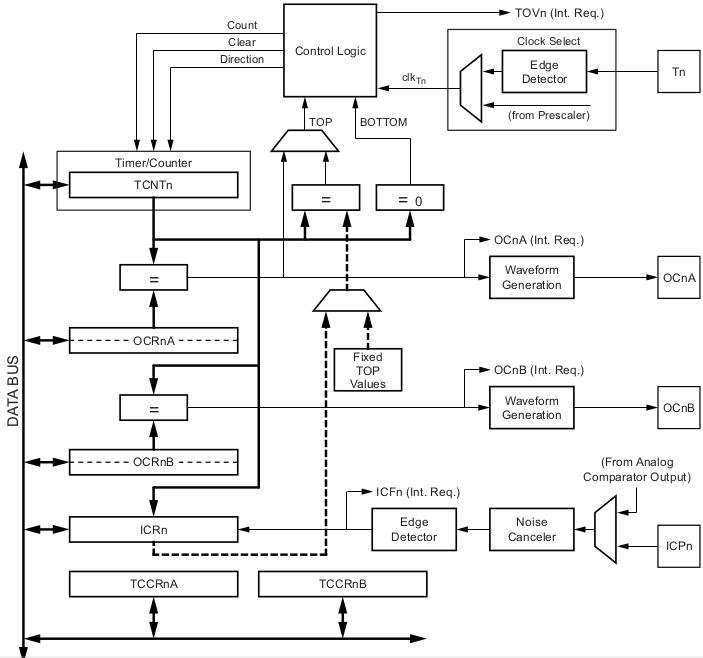
\includegraphics[height=0.6\textheight]{Timer1BlockDiagram.png}
    \end{center}
\end{figure}

\section{Terminologies and Registers}
\begin{minipage}{0.4\textwidth}
    \begin{tabular}{c|p{4.5cm}}
        \textbf{Parameter} & \textbf{Description}\\
        \hline
        BOTTOM & counter reaches 0x0000\\
        MAX & ounter reaches 0xFFFF\\
        TOP & counter reaches highest value (depends on mode of operation can be 0xFF, 0x1FF, 0x3FF, OCR1A, ICR1)
    \end{tabular}
\end{minipage}
\begin{minipage}{0.55\textwidth}
    \begin{tabular}{c|p{5.5cm}}
        \textbf{Register - 16 bit} & \textbf{Name}\\
        \hline
        \regFormat{TCN10} & Timer/Counter1count value\\
        \regFormat{TCCR1A} & Timer/Coutner1 Control Register A\\
        \regFormat{TCCR1B} & Timer/Coutner1 Control Register B\\
        \regFormat{OCBR1A} & Output compare register A\\
        \regFormat{OCBR1B} & Output compare register B\\
        \regFormat{TIFR1} & Timer Interrupt Flag Register\\
        \regFormat{TIMSK1} & Timer interrupt Mask Register\\
        \regFormat{ICR1} & Input Capture Register\\
    \end{tabular}
\end{minipage}

\textbf{Note: } 
\begin{itemize}
    \item The \regFormat{CNT1, OCR1A/B, ICR1} are 16-bit registers that can be accessed by the CPU via the 8-bit data bus.
    \item \textbf{For 16-bit write, the high byte must be written before the low byte.}
    \item \textbf{For 16-bit read, the low byte must be read before the high byte.}
\end{itemize}
\section{Timer/Counter1 Units}

\subsection{Clock Source/Select Unit}
\begin{figure}[H]
    \begin{center}
        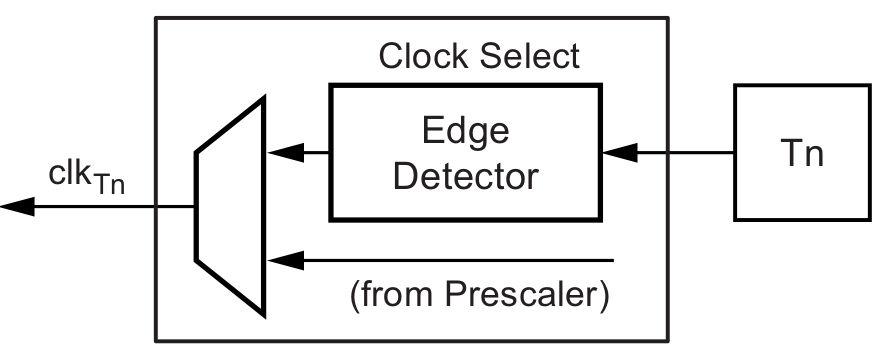
\includegraphics[width=0.5\textwidth]{Timer0ClockSelector.png}
    \end{center}
\end{figure}
\begin{itemize}
    \item The source for the Timer/Counter0 can be external or internal.
    \item External clock source is from \pinFormat{T1} pin.
    \item While Internal Clock source can be clocked via a prescalar.
    \item The output of this unit is the timer clock ($clk_{T1}$).
    \item It uses \bitFormat{CS1[2:0]} bits in \regFormat{TCCR1B} register to select the source.
\end{itemize}


\subsection{Counter Unit}
\begin{minipage}{0.5\textwidth}
    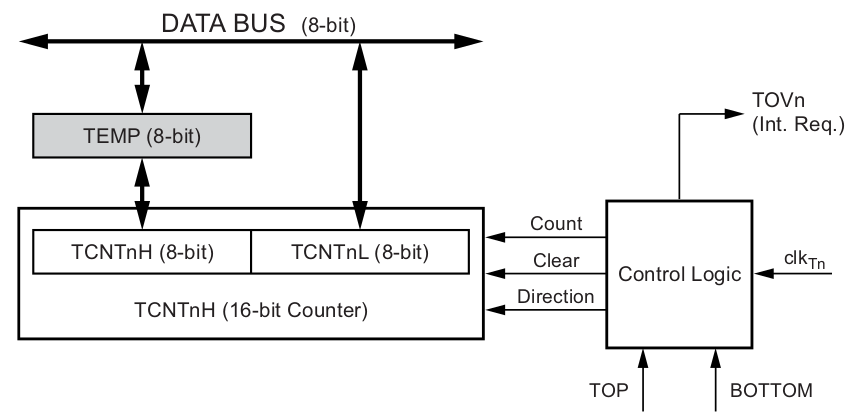
\includegraphics[width=1\textwidth]{Timer1CounterUnit.png}
\end{minipage}
\begin{minipage}{0.45\textwidth}
    \begin{tabular}{c|p{5.5cm}}
        \textbf{Signal} & \textbf{Description}\\
        \hline  
        count & Increment or decrement \regFormat{TCNT1} by 1\\
        direction & Select between increment or decrement\\
        clear & Clears \regFormat{TCNT1} to 0x0000\\
        $clk_{T1}$ & Timer/Coutner1 clock\\
        top & Signalize that \regFormat{TCNT1} has maximum value\\
        bottom & Signalize that \regFormat{TCNT1} has minimum value(0x0000)\\
    \end{tabular}
\end{minipage}
\begin{itemize}
    \item The main part of the 16-bit Timer/Counter is the programmable bi-directional counter.
    \item Counter high (\regFormat{TCNT1H}) containing the upper eight bits of the counter, and counter low (\regFormat{TCNT1L}) containing the lower eight bits.
    \item Depending the mode of operation the counter is cleared, incremented, or decremented at each timer clock ($clk_{T1}$).
    \item Counting sequence is determined by \bitFormat{WGM1[3:0]} bits of \regFormat{TCCR1A} -Timer/Counter1 Control register A and \regFormat{TCCR1B} - Timer/Counter1 Control register B.
    \item The Timer/Counter1 Overflow flag \bitFormat{(TOV1)} is set and can generate interrupt according to the mode.
\end{itemize}

\subsection{Input Capture Unit}
\begin{figure}[H]
    \centering
    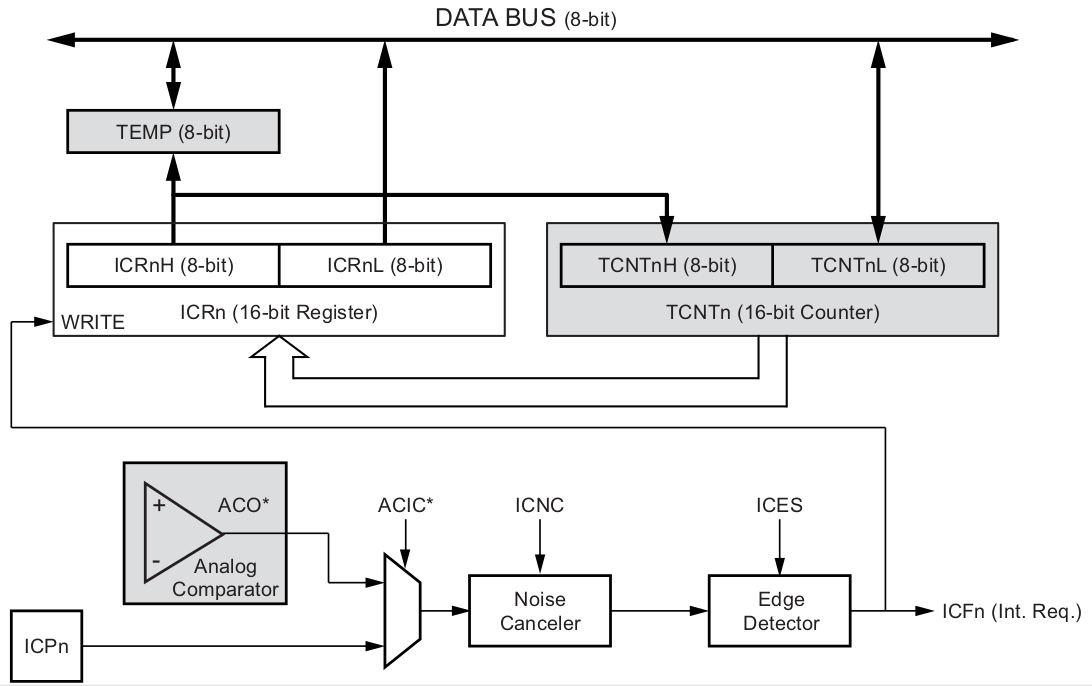
\includegraphics[width=0.75\textwidth]{Timer1InputCapture.png}
\end{figure}
\begin{itemize}
    \item Can capture external events and give them time-stamp indicating time of occurance.
    \item External signal can be from \pinFormat{ICP1} pin or analog-comparator unit.
    \item Usage : calculate frequency, duty-cycle, log of the signal
    \item When a change of the logic level (an event) occurs on the input capture pin (\pinFormat{ICP1}), or on the analog comparator output (\pinFormat{ACO)}, and this change confirms to the setting of the edge detector, a capture will be triggered. 
    \item When a capture is triggered, the 16-bit value of the counter (\regFormat{TCNT1}) is written to the input capture register (\regFormat{ICR1}).
    \item The input capture flag (\bitFormat{ICF1}) is set at the same system clock as the \regFormat{TCNT1} value is copied into \regFormat{ICR1} register. 
    \item If enabled (\bitFormat{ICIE1} = 1), the input capture flag generates an input capture interrupt.
    \item \bitFormat{ICF1} flag is automatically cleared when the interrupt is executed and by writing on to i.
    \item An input capture can be triggered by software by controlling the port of the \pinFormat{ICP1} pin.
\end{itemize}

\subsection{Output Compare Unit}
\begin{figure}[H]
    \begin{center}
        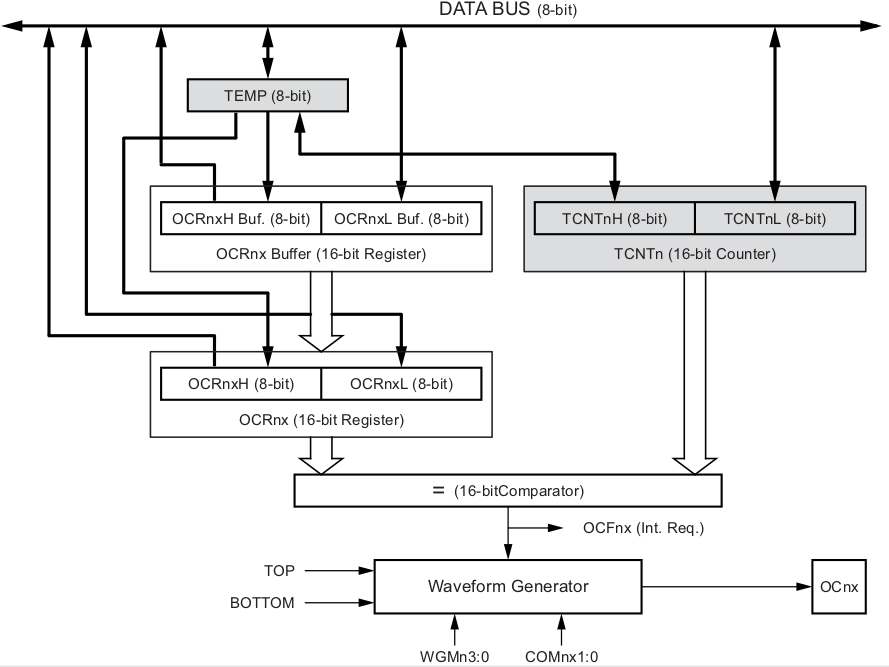
\includegraphics[width=0.6\textwidth]{Timer1OutputCompare.png}
    \end{center}
\end{figure}
\begin{itemize}
    \item 16-bit comparator continuously compares \regFormat{TCNT1} with both \regFormat{OCR1A} and \regFormat{OCR1B}.
    \item When \regFormat{TCNT1} equals \regFormat{OCR1A} or \regFormat{OCR1B}, the comparator signals a match which will set the output compare flag at the next timer clock cycle.
    \item If interrupts are enabled, then output compare interrupt is generated.
    \item The waveform generator uses the match signal to generate an output according to operating mode set by the \bitFormat{WGM1[3:0]} bits and compare output mode \bitFormat{COM0x[1:0]} bits.
\end{itemize}

\subsection{Compare Match Output Unit}
\begin{figure}[H]
    \begin{center}
        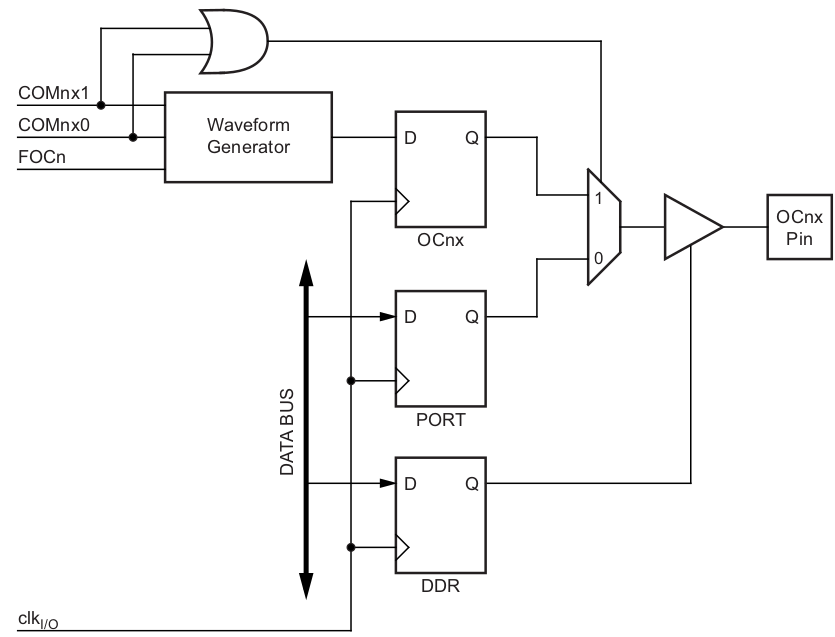
\includegraphics[height=0.3\textheight]{Timer1ComparteMatchOutput.png}
    \end{center}
\end{figure}
\begin{itemize}
    \item This unit is used for changing the state of \pinFormat{OC1A} and \pinFormat{OC1B} pins by configuring the \bitFormat{COM1x[1:0]} bits.
    \item But, general I/O port function is overriiden by DDR reigster.
\end{itemize}


\section{Modes of Operation}
\begin{itemize}
    \item The mode of operation can be defined by combination of waveform generation mode (\bitFormat{WGM1[3:0]}) and compare output mode(\bitFormat{COM1[1:0]}) bits.
    \item The waveform generation mode (\bitFormat{WGM1[3:0]}) bits affect the counting sequence.
    \item For non-PWM mode, \bitFormat{COM1[1:0]} bits control if the output should be set, cleared or toggled at a compare match.
    \item For PWM mode, \bitFormat{COM1[1:0]} bits control if the PWM generated should be inverted or non-inverted.
\end{itemize}



\subsection{Normal Mode - Non-PWM Mode}
\begin{itemize}
    \item \bitFormat{WGM1[3:0]} $-->$ 000.
    \item Counter counts up and no counter clear.
    \item Overruns TOP(0XFFFF) and restarts from BOTTOM(0X0000).
    \item \bitFormat{TOV1} Flag is only set when overrun.
    \item We have to clear \bitFormat{TOV1} flag inorder to have next running.
    \item But, if we use interrupt we don’t need to clear it as interrupt automatically clear the \bitFormat{TOV1} flag.
    \item The input capture unit can be used to capture events at \pinFormat{ICP1} pin or \pinFormat{ACO} pin.
    \item The timing can be seen below.
\end{itemize}

\begin{tikztimingtable}[
    timing/dslope=0.1,
    timing/.style={x=5ex,y=2ex},
    x=5ex,
    timing/rowdist=3ex,
    timing/name/.style={font=\sffamily\scriptsize}
    ]
    \busref{clk\_{T1}}  & 41{c}\\
    \busref{TCNT1} & u{} D{0x0000} D{0x0001};[dotted] 2D{};D{0xFFFE} D{0xFFFF}D{0x0000} D{0x0001};[dotted] 2D{};D{0xFFFE} D{0xFFFF}D{0x0000} D{0x0001};[dotted] 2D{};D{0xFFFE} D{0xFFFF}D{0x0000} D{0x0001}\\
    \busref{TOV1} & l 6{L} H 5{L} H 5{L} H 1{L}\\
\end{tikztimingtable}



\subsection{Clear Timer on Compare Match(CTC) Mode - Non-PWM Mode}
\begin{itemize}
    \item \bitFormat{WGM1[3:0]} $-->$ 0100 or 1100.
    \begin{itemize}
        \item Counter value clears when \regFormat{TCNT1} reaches \regFormat{OCR1A} if \bitFormat{WGM1[3:0]} is 0100.
        \item Counter value clears when \regFormat{TCNT1} reaches \regFormat{ICR1} if \bitFormat{WGM1[3:0]} is 1100.
    \end{itemize}
    \item Interrupt can be generated each time \regFormat{TCNT1} reaches \regFormat{OCR1A} register value by \bitFormat{OCF1A} flag.
    \item Interrupt can be generated each time \regFormat{TCNT1} reaches \regFormat{ICR1} register value by \bitFormat{ICF1} flag.
    \item When \bitFormat{COM1A[1:0]} == 01, the \pinFormat{OC1A} pin output can be set to toggle its match between \regFormat{TCNT1} and \regFormat{OCR1A} or \regFormat{ICR1} register to generate waveform.
    \item The frequency of the waveform its
    \begin{center}
        { \Large $f_{OC1A} = \frac{f_{clkT1}}{2 * N * (1 + OCR1A)}$ }
    \end{center}
    \item Here N is prescalar factor and can be (1, 8, 64, 256, or 1024).
\end{itemize}


\subsubsection{WGM1[3:0] == 0100}
\begin{tikztimingtable}[
    timing/dslope=0.1,
    timing/.style={x=5ex,y=2ex},
    x=5ex,
    timing/rowdist=3ex,
    timing/name/.style={font=\sffamily\scriptsize}
    ]
    \busref{clk\_{T1}}  & 28{1.5c}\\
    \busref{TCNT1} & 0.75U{} 1.5D{0x0000} 1.5D{0x0001};[dotted] 3D{};1.5D{OCR1A - 1} 1.5D{OCR1A}1.5D{0x0000} 1.5D{0x0001};[dotted] 3D{};1.5D{OCR1A - 1} 1.5D{OCR1A} 1.5D{0x0000} 0.75D{0x0001} \\
    \busref{OC1A} & 0.75L 9{L} 1.5H l 7{L} 1.5H l\\
\end{tikztimingtable}
\subsubsection{WGM1[3:0] == 1100}
\begin{tikztimingtable}[
    timing/dslope=0.1,
    timing/.style={x=5ex,y=2ex},
    x=5ex,
    timing/rowdist=3ex,
    timing/name/.style={font=\sffamily\scriptsize}
    ]
    \busref{clk\_{T1}}  & 28{1.5c}\\
    \busref{TCNT1} & 0.75U{} 1.5D{0x0000} 1.5D{0x0001};[dotted] 3D{};1.5D{ICR1 - 1} 1.5D{ICR1}1.5D{0x0000} 1.5D{0x0001};[dotted] 3D{};1.5D{ICR1 - 1} 1.5D{ICR1} 1.5D{0x0000} 0.75D{0x0001} \\
    \busref{OC1A} & 0.75L 9{L} 1.5H l 7{L} 1.5H l\\
\end{tikztimingtable}

\subsection{Fast PWM Mode}
\begin{itemize}
    \item \bitFormat{WGM1[3:0]} $-->$ 0101 or 0110 or 0111 or 1110 or 1111.
    \item Power Regulation, Rectification, DAC applications.
    \item Single slope operations causing high frequency PWM waveform.
    \item Counter starts from BOTTOM to TOP and then restarts from BOTTOM.
    \item TOP is defined by
    \begin{itemize}
        \item TOP == 0x00FF if \bitFormat{WGM1[3:0]} $-->$ 0101
        \item TOP == 0x01FF if \bitFormat{WGM1[3:0]} $-->$ 0110
        \item TOP == 0x03FF if \bitFormat{WGM1[3:0]} $-->$ 0111
        \item TOP ==   \regFormat{ICR1} if \bitFormat{WGM1[3:0]} $-->$ 1110
        \item TOP ==  \regFormat{OCR1A} if \bitFormat{WGM1[3:0]} $-->$ 1111
    \end{itemize}
    \item  When \bitFormat{COM1A[1:0]} == 01, the \pinFormat{OC1A} pin output can be set to toggle its match between \regFormat{TCNT1} and TOP to generate waveform.
    \begin{itemize}
        \item The above is possible only when \bitFormat{WGM12} bit is set.
        \item And only on \pinFormat{OC1A} pin and not on \pinFormat{OC1B} pin.
    \end{itemize}
    \item In Inverting Compare Mode \bitFormat{COM1A[1:0]} == 10 , the \pinFormat{OC1A} or \pinFormat{OC1B} pins is made 1 on compare match between \regFormat{TCNT1} and TOP and made 0 on reaching BOTTOM.
    \item In Non-Inverting Compare Mode \bitFormat{COM1A[1:0]} == 11 , the \pinFormat{OC1A} or \pinFormat{OC1B} pins is made 0 on compare match between \regFormat{TCNT1} and TOP and 1 made  on reaching BOTTOM.
    \item The Timer/Counter overflow flag (\bitFormat{TOV1}) is set each time the counter reaches TOP.
    \item The PWM frequency is given by 
    \begin{center}
        { \Large $f_{OC1xPWM} = \frac{f_{clkT1}}{N * (1+ TOP)}$ }
    \end{center}
\end{itemize}

\subsubsection{WGM1[3:0] == 0101}
\begin{tikztimingtable}[
    timing/dslope=0.1,
    timing/.style={x=5ex,y=2ex},
    x=5ex,
    timing/rowdist=3ex,
    timing/name/.style={font=\sffamily\scriptsize}
    ]
    \busref{clk\_{T0}}  & 41{1c} c\\
    \busref{TCNT1} & 0.5U{} D{0x0000} 1D{0x0001};[dotted] 1.5D{};1D{0x00FE} 1D{0x00FF}1D{0x0000} 1D{0x0001};[dotted] 1D{};1D{0x00FE} 1D{0x00FF} 1D{0x0000} 1D{0x0001} [dotted] 1D{};1D{0x00FE} 1D{0x00FF} 1D{0x0000} 1D{0x0001};[dotted] 1D{};1D{0x00FE} 1D{0x00FF};\\
    \busref{TOV1} & 6{L} H 4{L} H 4{L} H 4{L} \\
\end{tikztimingtable}

\subsubsection{WGM1[3:0] == 0110}
\begin{tikztimingtable}[
    timing/dslope=0.1,
    timing/.style={x=5ex,y=2ex},
    x=5ex,
    timing/rowdist=3ex,
    timing/name/.style={font=\sffamily\scriptsize}
    ]
    \busref{clk\_{T0}}  & 41{1c} c\\
    \busref{TCNT1} & 0.5U{} D{0x0000} 1D{0x0001};[dotted] 1.5D{};1D{0x01FE} 1D{0x01FF}1D{0x0000} 1D{0x0001};[dotted] 1D{};1D{0x01FE} 1D{0x01FF} 1D{0x0000} 1D{0x0001} [dotted] 1D{};1D{0x01FE} 1D{0x01FF} 1D{0x0000} 1D{0x0001};[dotted] 1D{};1D{0x01FE} 1D{0x01FF};\\
    \busref{TOV1} & 6{L} H 4{L} H 4{L} H 4{L} \\
\end{tikztimingtable}
\subsubsection{WGM1[3:0] == 0111}
\begin{tikztimingtable}[
    timing/dslope=0.1,
    timing/.style={x=5ex,y=2ex},
    x=5ex,
    timing/rowdist=3ex,
    timing/name/.style={font=\sffamily\scriptsize}
    ]
    \busref{clk\_{T0}}  & 41{1c} c\\
    \busref{TCNT1} & 0.5U{} D{0x0000} 1D{0x0001};[dotted] 1.5D{};1D{0x03FE} 1D{0x03FF}1D{0x0000} 1D{0x0001};[dotted] 1D{};1D{0x03FE} 1D{0x03FF} 1D{0x0000} 1D{0x0001} [dotted] 1D{};1D{0x03FE} 1D{0x03FF} 1D{0x0000} 1D{0x0001};[dotted] 1D{};1D{0x03FE} 1D{0x03FF};\\
    \busref{TOV1} & 6{L} H 4{L} H 4{L} H 4{L} \\
\end{tikztimingtable}

\subsubsection{WGM1[3:0] == 1110}
\begin{tikztimingtable}[
    timing/dslope=0.1,
    timing/.style={x=5ex,y=2ex},
    x=5ex,
    timing/rowdist=3ex,
    timing/name/.style={font=\sffamily\scriptsize}
    ]
    \busref{clk\_{T0}}  & 41{1c} c\\
    \busref{TCNT1} & 0.5U{} D{0x0000} 1D{0x001};[dotted] 1.5D{};1D{\tiny ICR1 -1} 1D{\tiny ICR1}1D{0x0000} 1D{0x0001};[dotted] 1D{};1D{\tiny ICR1 -1} 1D{\tiny ICR1} 1D{0x0000} 1D{0x0001} [dotted] 1D{};1D{\tiny ICR1 -1} 1D{\tiny ICR1} 1D{0x0000} 1D{0x0001};[dotted] 1D{};1D{\tiny ICR1 -1} 1D{\tiny ICR1};\\
    \busref{TOV1} & 6{L} H 4{L} H 4{L} H 4{L} \\
\end{tikztimingtable}

\subsubsection{WGM1[3:0] == 1111}
\begin{tikztimingtable}[
    timing/dslope=0.1,
    timing/.style={x=5ex,y=2ex},
    x=5ex,
    timing/rowdist=3ex,
    timing/name/.style={font=\sffamily\scriptsize}
    ]
    \busref{clk\_{T0}}  & 41{1c} c\\
    \busref{TCNT1} & 0.5U{} D{0x0000} 1D{0x001};[dotted] 1.5D{};1D{\tiny OCR1A -1} 1D{\tiny OCR1A}1D{0x0000} 1D{0x0001};[dotted] 1D{};1D{\tiny OCR1A -1} 1D{\tiny OCR1A} 1D{0x0000} 1D{0x0001} [dotted] 1D{};1D{\tiny OCR1A -1} 1D{\tiny OCR1A} 1D{0x0000} 1D{0x0001};[dotted] 1D{};1D{\tiny OCR1A -1} 1D{\tiny OCR1A};\\
    \busref{TOV1} & 6{L} H 4{L} H 4{L} H 4{L} \\
\end{tikztimingtable}

\subsection{Phase Correct PWM Mode}
\begin{itemize}
    \item \bitFormat{WGM1[3:0]} $-->$ 0001 or 0010 or 0011 or 1010 or 1011.    
    \item High resolution phase correct PWM.
    \item Motor control due to symmetric features
    \item Dual slope operations causing ower frequency PWM waveform.
    \item Counter starts from BOTTOM to TOP and then from TOP to BOTTOM.
    \item TOP is defined by
    \begin{itemize}
        \item TOP == 0x00FF if \bitFormat{WGM1[3:0]} $-->$ 0001
        \item TOP == 0x01FF if \bitFormat{WGM1[3:0]} $-->$ 0010
        \item TOP == 0x03FF if \bitFormat{WGM1[3:0]} $-->$ 0011
        \item TOP ==   \regFormat{ICR1} if \bitFormat{WGM1[3:0]} $-->$ 1010
        \item TOP ==  \regFormat{OCR1A} if \bitFormat{WGM1[3:0]} $-->$ 1011
    \end{itemize}
    \item  When \bitFormat{COM1A[1:0]} == 01, the \pinFormat{OC1A} pin output can be set to toggle its match between \regFormat{TCNT1} and TOP to generate waveform.
    \begin{itemize}
        \item The above is possible only when \bitFormat{WGM12} bit is set.
        \item And only on \pinFormat{OC1A} pin and not on \pinFormat{OC1B} pin.
    \end{itemize}
    \item In Inverting Compare Mode \bitFormat{COM1A[1:0]} == 10 , the \pinFormat{OC1A} or \pinFormat{OC1B} pins is made 1 on compare match between \regFormat{TCNT1} and TOP and made 0 on reaching BOTTOM.
    \item In Non-Inverting Compare Mode \bitFormat{COM1A[1:0]} == 11 , the \pinFormat{OC1A} or \pinFormat{OC1B} pins is made 0 on compare match between \regFormat{TCNT1} and TOP and 1 made  on reaching BOTTOM.
    \item The Timer/Counter overflow flag (\bitFormat{TOV1}) is set each time the counter reaches BOTTOM..
    \item The PWM frequency is given by 
    \begin{center}
        { \Large $f_{OC1xPWM} = \frac{f_{clkT1}}{2 * N * TOP}$ }
    \end{center}
\end{itemize}


\subsubsection{WGM1[3:0] == 0001}
\begin{tikztimingtable}[
    timing/dslope=0.1,
    timing/.style={x=5ex,y=2ex},
    x=5ex,
    timing/rowdist=3ex,
    timing/name/.style={font=\sffamily\scriptsize}
    ]
    \busref{clk\_{T1}}  & 41{1c} c\\
    \busref{TCNT1} & 0.5U{} D{0x0000} 1D{0x0001};[dotted] 1.5D{};1D{0x00FE} 1D{0x00FF}1D{0x0000} 1D{0x0001};[dotted] 1D{};1D{0x00FE} 1D{0x00FF} 1D{0x0000} 1D{0x0001} [dotted] 1D{};1D{0x00FE} 1D{0x00FF} 1D{0x0000} 1D{0x0001};[dotted] 1D{};1D{0x00FE} 1D{0x00FF};\\
    \busref{TOV1} & 6{L} H 4{L} H 4{L} H 4{L} \\
\end{tikztimingtable}


\subsubsection{WGM1[3:0] == 0010}
\begin{tikztimingtable}[
    timing/dslope=0.1,
    timing/.style={x=5ex,y=2ex},
    x=5ex,
    timing/rowdist=3ex,
    timing/name/.style={font=\sffamily\scriptsize}
    ]
    \busref{clk\_{T1}}  & 41{1c} c\\
    \busref{TCNT1} & 0.5U{} D{0x0000} 1D{0x0001};[dotted] 1.5D{};1D{0x01FE} 1D{0x01FF}1D{0x0000} 1D{0x0001};[dotted] 1D{};1D{0x01FE} 1D{0x01FF} 1D{0x0000} 1D{0x0001} [dotted] 1D{};1D{0x01FE} 1D{0x01FF} 1D{0x0000} 1D{0x0001};[dotted] 1D{};1D{0x01FE} 1D{0x01FF};\\
    \busref{TOV1} & 6{L} H 4{L} H 4{L} H 4{L} \\
\end{tikztimingtable}

\subsubsection{WGM1[3:0] == 0011}
\begin{tikztimingtable}[
    timing/dslope=0.1,
    timing/.style={x=5ex,y=2ex},
    x=5ex,
    timing/rowdist=3ex,
    timing/name/.style={font=\sffamily\scriptsize}
    ]
    \busref{clk\_{T1}}  & 41{1c} c\\
    \busref{TCNT1} & 0.5U{} D{0x0000} 1D{0x0001};[dotted] 1.5D{};1D{0x03FE} 1D{0x03FF}1D{0x0000} 1D{0x0001};[dotted] 1D{};1D{0x03FE} 1D{0x03FF} 1D{0x0000} 1D{0x0001} [dotted] 1D{};1D{0x03FE} 1D{0x03FF} 1D{0x0000} 1D{0x0001};[dotted] 1D{};1D{0x03FE} 1D{0x03FF};\\
    \busref{TOV1} & 6{L} H 4{L} H 4{L} H 4{L} \\
\end{tikztimingtable}

\subsubsection{WGM[2:0] == 1010}
\begin{tikztimingtable}[
    timing/dslope=0.1,
    timing/.style={x=5ex,y=2ex},
    x=5ex,
    timing/rowdist=3ex,
    timing/name/.style={font=\sffamily\scriptsize}
    ]
    \busref{clk\_{T1}}  & 41{1c}\\
    \busref{TCNT1} & 0.5U{} D{0x0000} 1D{0x0001};[dotted] 1.5D{};1D{\tiny OCR1A - 1} 1D{\tiny OCR1A}1D{\tiny OCR01-1} 1D{\tiny OCR1A-2};[dotted] 1D{};1D{0x0001} 1D{0x0000} 1D{0x0001}[dotted] 1D{};1D{\tiny OCR1A-1} 1D{\tiny OCR1A} 1D{\tiny OCR1A-1} 1D{\tiny OCR1A-2};[dotted] 1D{};1D{0x0001} 1D{0x0000} 1d{0x0001};\\
    \busref{TOV1} & l H l 8{L} H 8{L} H l\\
\end{tikztimingtable}

\subsubsection{WGM[2:0] == 1011}
\begin{tikztimingtable}[
    timing/dslope=0.1,
    timing/.style={x=5ex,y=2ex},
    x=5ex,
    timing/rowdist=3ex,
    timing/name/.style={font=\sffamily\scriptsize}
    ]
    \busref{clk\_{T1}}  & 41{1c}\\
    \busref{TCNT1} & 0.5U{} D{0x0000} 1D{0x0001};[dotted] 1.5D{};1D{\tiny ICR1- 1} 1D{\tiny ICR1}1D{\tiny ICR1-1} 1D{\tiny ICR1-2};[dotted] 1D{};1D{0x0001} 1D{0x0000} 1D{0x0001}[dotted] 1D{};1D{\tiny ICR1-1} 1D{\tiny ICR1} 1D{\tiny ICR1-1} 1D{\tiny ICR1-2};[dotted] 1D{};1D{0x0001} 1D{0x0000} 1d{0x0001};\\
    \busref{TOV1} & l H l 8{L} H 8{L} H l\\
\end{tikztimingtable}

\subsection{Phase and Frequency Corrected PWM Mode}
\begin{itemize}
    \item \bitFormat{WGM1[3:0]} $-->$ 1000 or 1001.
    \item High resolution and Phase correctd PWM.
    \item Dual-Slope.
    \item Counter counts from BOTTOM to TOP and then from TOP to BOTTOM.
    \begin{itemize}
        \item TOP == \regFormat{OCR1A} if \bitFormat{WGM1[3:0]} $-->$ 1001
        \item TOP == \regFormat{ICR1} if \bitFormat{WGM1[3:0]} $-->$ 1000
    \end{itemize}
    \item In Inverting Compare Mode \bitFormat{COM1x[1:0]} == 10 the \pinFormat{OC0x} pins is made 1 on compare match between \regFormat{TCNT1} and TOP when upcounting and made 0 on compare match between \regFormat{TCNT1} and TOP when downcounting.
    \item In Non-Inverting Compare Mode \bitFormat{COM1x[1:0]} == 11, the \pinFormat{OC0x} pins is made 0 on compare match between \regFormat{TCNT1} and TOP when upcounting AND made 1 on compare match between \regFormat{TCNT1} and TOP when downcounting.
    \item The Timer/Counter overflow flag (\bitFormat{TOV1}) is set each time the counter reaches BOTTOM.
    \item The interrupt flag can be used to generate an interrupt each time the counter reaches the BOTTOM value.
    \item The PWM frequency is given by 
    \begin{center}
        { \Large $f_{OC1xPWM} = \frac{f_{clkT1}}{2 * N * TOP}$ }
    \end{center}
\end{itemize}
\newpage

\section{Register Description}
\subsubsection*{TCCR1A – Timer/Counter 1 Control Register A}
\vspace*{0.5cm}
\begin{bytefield}[bitformatting={\large\bfseries},
    endianness=big,bitwidth=0.125\linewidth]{8}
    \bitheader[lsb=0]{0-7} \\
    \bitbox{1}{\small COM1A1}
    \bitbox{1}{\small COM1A0}
    \bitbox{1}{\small COM1B1}
    \bitbox{1}{\small COM1B0}
    \bitbox{1}{\small -}
    \bitbox{1}{\small -}
    \bitbox{1}{\small WGM11}
    \bitbox{1}{\small WGM10}\\
\end{bytefield}

\begin{table}[H]
    \begin{center}
        \begin{tabular}{c|p{4.1cm}|p{4.5cm}|p{4.9cm}}
            \bitFormat{COM1x[1:0]} & \textbf{Non-PWM modes} & \textbf{Fast PWM} & \textbf{Phase Corrected PWM \& Phase and Frequency Corrected PWM}\\
            \hline
            00 & No output @ \pinFormat{PB1 - OC1A} or \pinFormat{PB2 - OC1B} pin &   No output @ \pinFormat{PB1 - OC1A} or \pinFormat{PB2 - OC1B} pin & No output @ \pinFormat{PB1 - OC1A} or \pinFormat{PB2 - OC1B} pin \\
            \hline
            01 &  Toggle \pinFormat{PB1 - OC1A} or \pinFormat{PB2 - OC1B} pin on compare Match. & When \bitFormat{WGM[3:0]} == 1110 or 1111, Toggle \pinFormat{OC1A} pin on compare match & When \bitFormat{WGM[3:0]} == 1110 or 1111, Toggle \pinFormat{OC1A} pin on comapre match.\\
            \hline
            10 & Clear \pinFormat{PB1 - OC1A} or \pinFormat{PB2 - OC1B} pin on compare Match. & Clear \pinFormat{PB1 - OC1A} or \pinFormat{PB2 - OC1B} on compare match and  set \pinFormat{PB1 - OC1A} or \pinFormat{PB2 - OC1B} at BOTTOM & Clear \pinFormat{PD5 - OC0B} on compare match when up-counting and set \pinFormat{PB1 - OC1A} or \pinFormat{PB2 - OC1B} on compare match when down-counting.\\
            \hline
            11 & Set \pinFormat{PB1 - OC1A} or \pinFormat{PB2 - OC1B} pin on compare Match. & Set \pinFormat{PB1 - OC1A} or \pinFormat{PB2 - OC1B} on compare match and clear \pinFormat{PB1 - OC1A} or \pinFormat{PB2 - OC1B} at BOTTOM & Set \pinFormat{PD5 - OC0B} on compare match when up-counting and clear \pinFormat{PB1 - OC1A} or \pinFormat{PB2 - OC1B} on compare match when down-counting.\\
        \end{tabular}
    \end{center}
\end{table}


\begin{table}[H]
    \begin{center}
        \begin{tabular}{c|c|c|c}
            \bitFormat{WGM1[3:0]} & \textbf{Mode of operation} & \textbf{TOP} & \textbf{TOV1 Flag set on}\\
            \hline
            0000 & Normal & 0xFFFF & MAX\\
            0001 & PWM Phase corrected – 8bit & 0x00FF & BOTTOM\\
            0010 & PWM Phase corrected – 9bit & 0x01FF & BOTTOM\\
            0011 & PWM Phase corrected – 10bit & 0x03FF & BOTTOM\\
            0100 & CTC & OCR1A & MAX\\
            0101 & Fast PWM – 8bit & 0x00FF & TOP\\
            0110 & Fast PWM – 9bit & 0x01FF & TOP\\
            0111 & Fast PWM – 10bit & 0x03FF & TOP\\
            1000 & PWM, phase and frequency corrected & ICR1 & BOTTOM\\
            1001 & PWM, phase and frequency corrected & OCR1A & BOTTOM\\
            1010 & PWM, phase corrected & ICR1 & BOTTOM\\
            1011 & PWM, phase corrected & OCR1A & BOTTOM\\
            1100 & CTC & ICR1 & MAX\\
            1110 & Fast PWM & ICR1 & TOP\\
            1111 & Fast PWM & OCR1A & TOP\\
        \end{tabular}
    \end{center}
\end{table}

\subsubsection*{TCCR1B – Timer/Counter1 Control Register B}
\vspace*{0.5cm}
\begin{bytefield}[bitformatting={\large\bfseries},
    endianness=big,bitwidth=0.125\linewidth]{8}
    \bitheader[lsb=0]{0-7} \\
    \bitbox{1}{\small ICNC1}
    \bitbox{1}{\small ICES1}
    \bitbox{1}{\small -}
    \bitbox{1}{\small WGM13}
    \bitbox{1}{\small WGM12}
    \bitbox{1}{\small CS12}
    \bitbox{1}{\small CS11}
    \bitbox{1}{\small CS10}\\
\end{bytefield}
\begin{itemize}
    \item \bitFormat{ICNC1 - Input Capture Noise Canceler} - activates the input capture noise canceler.
    \item \bitFormat{ICES1 - Input Capture Edge Select} - selects which edge on the input capture pin (\pinFormat{ICP1}) that is used to trigger a capture event. [1 - Rising edge; 0 - falling edge;]
\end{itemize}

\begin{table}[H]
    \begin{center}
        \begin{tabular}{c|c}
            \bitFormat{CS1[2:0]} & \textbf{Description(Prescalar)}\\
            \hline
            000 & No clock source(Timer/Counter Stopped)\\
            001 & $clk_{I/O}$ – no prescaling\\
            010 & $\frac{clk_{I/O}}{8}$\\
            011 & $\frac{clk_{I/O}}{64}$\\\
            100 & $\frac{clk_{I/O}}{256}$\\\
            101 & $\frac{clk_{I/O}}{1024}$\\\
            110 & External clock source on \pinFormat{T1} pin. Clock on falling edge.\\
            111 & External clock source on \pinFormat{T1} pin. Clock on rising edge.\\
        \end{tabular}
    \end{center}
\end{table}

\subsubsection*{TCNT1H – Timer/Counter1 Counter Higher Byte}
\vspace*{0.5cm}
\begin{bytefield}[bitformatting={\large\bfseries},
    endianness=big,bitwidth=0.125\linewidth]{8}
    \bitheader[lsb=0]{0-7} \\
    \bitbox{8}{TCNT1[15:8]}\\
\end{bytefield}
\subsubsection*{TCNT1L – Timer/Counter1 Counter Lower Byte}
\vspace*{0.5cm}
\begin{bytefield}[bitformatting={\large\bfseries},
    endianness=big,bitwidth=0.125\linewidth]{8}
    \bitheader[lsb=0]{0-7} \\
    \bitbox{8}{TCNT1[7:0]}\\
\end{bytefield}

\subsubsection*{OCR1AH – Output Compare Register 1 A Higher Byte}
\vspace*{0.5cm}
\begin{bytefield}[bitformatting={\large\bfseries},
    endianness=big,bitwidth=0.125\linewidth]{8}
    \bitheader[lsb=0]{0-7} \\
    \bitbox{8}{OCR1A[15:8]}\\
\end{bytefield}
\subsubsection*{OCR1AL – Output Compare Register 1 A Lower Byte}
\vspace*{0.5cm}
\begin{bytefield}[bitformatting={\large\bfseries},
    endianness=big,bitwidth=0.125\linewidth]{8}
    \bitheader[lsb=0]{0-7} \\
    \bitbox{8}{OCR1A[7:0]}\\
\end{bytefield}

\subsubsection*{OCR1BH – Output Compare Register 1 B Higher Byte}
\vspace*{0.5cm}
\begin{bytefield}[bitformatting={\large\bfseries},
    endianness=big,bitwidth=0.125\linewidth]{8}
    \bitheader[lsb=0]{0-7} \\
    \bitbox{8}{OCR1B[15:8]}\\
\end{bytefield}
\subsubsection*{OCR1BL – Output Compare Register 1 B Lower Byte}
\vspace*{0.5cm}
\begin{bytefield}[bitformatting={\large\bfseries},
    endianness=big,bitwidth=0.125\linewidth]{8}
    \bitheader[lsb=0]{0-7} \\
    \bitbox{8}{OCR1B[7:0]}\\
\end{bytefield}

\subsubsection*{ICR1H – Input Capture Register 1 Higher Byte}
\vspace*{0.5cm}
\begin{bytefield}[bitformatting={\large\bfseries},
    endianness=big,bitwidth=0.125\linewidth]{8}
    \bitheader[lsb=0]{0-7} \\
    \bitbox{8}{ICR1[15:8]}\\
\end{bytefield}
\subsubsection*{ICR1L – Input Capture Register 1 Lower Byte}
\vspace*{0.5cm}
\begin{bytefield}[bitformatting={\large\bfseries},
    endianness=big,bitwidth=0.125\linewidth]{8}
    \bitheader[lsb=0]{0-7} \\
    \bitbox{8}{ICR1[7:0]}\\
\end{bytefield}

\subsubsection*{TIMSK1 – Timer/Counter 1 Interrupt Mask Register}
\vspace*{0.5cm}
\begin{bytefield}[bitformatting={\large\bfseries},
    endianness=big,bitwidth=0.125\linewidth]{8}
    \bitheader[lsb=0]{0-7} \\
    \bitbox{1}{\small -}
    \bitbox{1}{\small -}
    \bitbox{1}{\small ICIE1}
    \bitbox{1}{\small -}
    \bitbox{1}{\small -}
    \bitbox{1}{\small OCIE1B}
    \bitbox{1}{\small OCIE1A}
    \bitbox{1}{\small TOIE1}\\
\end{bytefield}

\quad Enable interrupts for compare match between \regFormat{TCNT1} and \regFormat{OCR1A} or \regFormat{TCNT1} and \regFormat{OCR1B} or overflow in \regFormat{TCNT1} or Input capture interrupt enable.


\subsubsection*{TIFR1 – Timer/Counter 1 Interrupt Flag Register}
\vspace*{0.5cm}
\begin{bytefield}[bitformatting={\large\bfseries},
    endianness=big,bitwidth=0.125\linewidth]{8}
    \bitheader[lsb=0]{0-7} \\
    \bitbox{1}{\small -}
    \bitbox{1}{\small -}
    \bitbox{1}{\small ICF1}
    \bitbox{1}{\small -}
    \bitbox{1}{\small -}
    \bitbox{1}{\small OCIE1B}
    \bitbox{1}{\small OCIE1A}
    \bitbox{1}{\small TOIE1}\\
\end{bytefield}

\quad Flag registers for interrupts on compare match between \regFormat{TCNT0} and \regFormat{OCR0A} or \regFormat{TCNT0} and \regFormat{OCR0B} or overflow in \regFormat{TCNT1} or capture event occurs on the \pinFormat{ICP1} pin .


\section{Configuring the Timer/Counter}
\subsection{Normal Mode}
\subsubsection{As Timer}
\begin{center}
    $ON\_TIME = \frac{max\_count}{\frac{F\_CPU}{PRESCALAR}}$
\end{center}
\begin{itemize}
    \item Depending on PRESCALR value, we get different ON\_TIME.
    \item First, \bitFormat{WGM1[3:0]} bits are configured as 0000 for Normal Mode in \regFormat{TCCR1A} and \regFormat{TCCR1B} registers.
    \item Next, \bitFormat{COM1A[1:0]} and/or \bitFormat{COM1A[1:0]} bits are configured to make outputs \pinFormat{OC1A} and/or \pinFormat{OC1B} pins to do nothing, set, clear or toggle in \regFormat{TCCR1A} register.
    \item Next, Interrupt is Enabled by \bitFormat{TOIE1} (overflow enable) in \regFormat{TIMSK1} reigster.
    \item Finally, Timer is started by setting prescalar in \bitFormat{CS1[2:0]} bits as needed prescalar of \regFormat{TCR1B} reigster.
    \item Global Interrupt is enabled.
    \item A interrupt Service Routine for Timer1 overflow is Written.
    \item No need to clear the overflow flag as it is done by hardware.
    \item The timing when both pins \pinFormat{OC1A} and \pinFormat{OC1B} are made to toggle.
\end{itemize}

\begin{tikztimingtable}[
    timing/dslope=0.1,
    timing/.style={x=5ex,y=2ex},
    x=5ex,
    timing/rowdist=3ex,
    timing/name/.style={font=\sffamily\scriptsize}
    ]
    \busref{clk\_{T1}}  & 41{c}\\
    \busref{TCNT1} & u{} D{0x0000} D{0x0001};[dotted] 2D{};D{0xFFFE} D{0xFFFF}D{0x0000} D{0x0001};[dotted] 2D{};D{0xFFFE} D{0xFF}D{0x0000} D{0x0001};[dotted] 2D{};D{0xFFFE} D{0xFFFF}D{0x0000} D{0x0001}\\
    \busref{TOV1} & u h h 5{L} H 5{L} H 5{L} H 1{L}\\
    \busref{OC1A} & l H 5{H} 6{L} 6{H} 2{L}\\
    \busref{OC1B} & h L 5{L} 6{H} 6{L} 2{H}\\
\end{tikztimingtable}
\begin{itemize}
    \item The code can be seen below,
\end{itemize}
\begin{minted}[breaklines, bgcolor=lightgray]{c}
// MOde of operation to Normal Mode -- WGM1[3:0] === 0000
// WGM1[3](bit4) from TCCR1B, WGM1[2](bit3) from TCCR1B, WGM1[1](bit1)  from TCC1RA, WGM1[0](bit0)  from TCCR1A	
TCCR1A = TCCR1A & ~(1<<WGM10);
TCCR1A = TCCR1A & ~(1<<WGM11);
TCCR1B = TCCR1B & ~(1<<WGM12);
TCCR1B = TCCR1B & ~(1<<WGM13);

/* What to do when timer reaches the MAX(0xFFFF) value */
// toggle OC1A on each time when reaches the MAX(0xFFFF)
// which is reflected in PB1
// Output OC1A to toglle when reaches MAX -- COM1A[1:0] === 01
// COM1A[1](bit7) from TCCR1A, COM1A[0](bit6) from TCCR1A
TCCR1A = TCCR1A & ~(1<<COM1A1);
TCCR1A = TCCR1A | (1<<COM1A0);

// toggle OC1B on each time when reaches the MAX(0xFFFF)
// which is reflected in PB2
// Output OC1B to toglle when reaches MAX -- COM1B[:0] === 01
// COM1B[1](bit5) from TCCR1A, COM1B[0](bit4) from TCCR1A
TCCR1A = TCCR1A & ~(1<<COM1B1);
TCCR1A = TCCR1A | (1<<COM1B0);


//Enable Interrupt of OVERFLOW flag so that interrupt can be generated
TIMSK1 = TIMSK1 | (1<<TOV1);

// start timer by setting the clock prescalar
// SAME AS from I/O clock
// same-- CS1[2:0] === 001
// CS1[2](bit2) from TCCR1B,CS1[1](bit1) from TCCR1B,CS1[0](bit0) from TCCR1B
TCCR1B = TCCR1B | (1<<CS10);
TCCR1B = TCCR1B & ~(1<<CS11);
TCCR1B = TCCR1B & ~(1<<CS12);

// enabling global interrupt

sei();
// SO ON TIME = max_count / (F_CPU / PRESCALAR)
// ON TIME = 0xFFFF / (16000000/1) = 4.096ms
// since symmetric as toggling OFF TIME = 4.096ms
// hence, we get a square wave of fequency 1 / 8.192ms = 122.07Hz
\end{minted}


\subsubsection{As Counter}
\begin{itemize}
    \item Every rising/falling edge the count increases.
    \item So to reach 0xFFFF count, it would take a time of $\frac{0xFFFF}{frequency @ \pinFormat{T1} pin}$.
    \item First, \bitFormat{WGM1[3:0]} bits are configured as 0000 for Normal Mode in \regFormat{TCCR1A} and \regFormat{TCCR1B} registers.
    \item Finally, Counter is started by configuring \bitFormat{CS1[2:0]} bits to 110 or 111 for external falling or rising edge on \pinFormat{T1 - PD5}.
    \item The code when \pinFormat{T1} pin is used as counter @ falling edge.
\end{itemize}
\begin{minted}[breaklines,bgcolor=lightgray]{c}
// MOde of operation to Normal Mode -- WGM1[3:0] === 0000
// WGM1[3](bit4) from TCCR1B, WGM1[2](bit3) from TCCR1B, WGM1[1](bit1)  from TCC1RA, WGM1[0](bit0)  from TCCR1A	
TCCR1A = TCCR1A & ~(1<<WGM10);
TCCR1A = TCCR1A & ~(1<<WGM11);
TCCR1B = TCCR1B & ~(1<<WGM12);
TCCR1B = TCCR1B & ~(1<<WGM13);
    
/* to count external event -we must connect source to T1 (PD5) */
// THE CLK IS CLOCKED FROM external source
// Falling edge of T1(PD5) -- CS1[2:0] === 110
// CS1[2](bit2) from TCCR1B,CS1[1](bit1) from TCCR1B,CS1[0](bit0) from TCCR1B
TCCR1B = TCCR1B & ~(1<<CS10);
TCCR1B = TCCR1B | (1<<CS11);
TCCR1B = TCCR1B | (1<<CS12);
\end{minted}

\subsubsection{As Input Capture}
\begin{itemize}
    \item Capture the value of \regFormat{TCNT1} into \regFormat{ICR1} register when there is rising or falling edge.
    \item First, \bitFormat{WGM1[3:0]} bits are configured as 0000 for Normal Mode in \regFormat{TCCR1A} and \regFormat{TCCR1B} registers.
    \item Next, the falling or rising edge for the \pinFormat{ICP1} pin is selected by \bitFormat{ICES1} bit in \regFormat{TCCR1B}.
    \item The interrupts for input capture is enabled by setting the \bitFormat{ICIE1} bit in \regFormat{TIMSK1}.
    \item A interrupt service routing is written.
    \item Finally, Timer is started by setting prescalar in \bitFormat{CS1[2:0]} bits as needed prescalar of \regFormat{TCR1B} reigster.
    \item The code when \pinFormat{ICP1 - PB0} pin is used as capture @ rising edge.
\end{itemize}
\begin{minted}[breaklines,bgcolor=lightgray]{c}
// MOde of operation to Normal Mode -- WGM1[3:0] === 0000
// WGM1[3](bit4) from TCCR1B, WGM1[2](bit3) from TCCR1B, WGM1[1](bit1)  from TCC1RA, WGM1[0](bit0)  from TCCR1A	
TCCR1A = TCCR1A & ~(1<<WGM10);
TCCR1A = TCCR1A & ~(1<<WGM11);
TCCR1B = TCCR1B & ~(1<<WGM12);
TCCR1B = TCCR1B & ~(1<<WGM13);

// Select the edge for Input Capture
// ICES1(bit6) from TCCR1B
// Capture on Rising edge, ICES1 === 1
TCCR1B |= (1<<ICES1);

//Enable Interrupt of Input Capture Interrupt Enable so that interrupt can be generated
TIMSK1 = TIMSK1 | (1<<ICIE1);
    
// start timer by setting the clock prescalar
// SAME AS from I/O clock
// same-- CS1[2:0] === 001
// CS1[2](bit2) from TCCR1B,CS1[1](bit1) from TCCR1B,CS1[0](bit0) from TCCR1B
TCCR1B = TCCR1B | (1<<CS10);
TCCR1B = TCCR1B & ~(1<<CS11);
TCCR1B = TCCR1B & ~(1<<CS12);

// enabling global interrupt

sei();

ISR(TIMER1_CAPT_vect)
{
	if((TIFR1 & (1<<ICF1)) != 0)
	{
		capVal = ICR1L;
		capVal = (ICR1H<<8) | (capVal & 0xFF);
		// see datamemory
	}
}
\end{minted}


\subsubsection{Application I - Delay}
\begin{minted}[breaklines,bgcolor=lightgray]{c}
/* TCNT1 starts from 0X0000 goes upto 0XFFFF and restarts */
/* No possible use case as it just goes upto 0xFFFF and restarts */
// MOde of operation to Normal Mode -- WGM1[3:0] === 0000
// WGM1[3](bit4) from TCCR1B, WGM1[2](bit3) from TCCR1B, WGM1[1](bit1)  from TCC1RA, WGM1[0](bit0)  from TCCR1A	
TCCR1A = TCCR1A & ~(1<<WGM10);
TCCR1A = TCCR1A & ~(1<<WGM11);
TCCR1B = TCCR1B & ~(1<<WGM12);
TCCR1B = TCCR1B & ~(1<<WGM13);

/* What to do when timer reaches the MAX(0xFFFF) value */
// nothing should be done on OC1A for delay
// nothing  -- COM1A[1:0] === 00
// COM1A[1](bit7) from TCCR1A, COM1A[0](bit6) from TCCR1A
TCCR1A = TCCR1A & ~(1<<COM1A1);
TCCR1A = TCCR1A & ~(1<<COM1A0);
    
/* The delay possible = 0xffff / (F_CPU/prescalar) */
// lowest delay = 0xffff / (16000000 / 1) = 4.096ms
// when prescalar == 8 --> delay = 0xffff / (16000000 / 8) = 32.768ms
// when prescalar == 64 --> delay = 0xffff / (16000000 / 64) = 262.144ms
// when prescalar == 256 --> delay = 0xffff / (16000000 / 256) = 1.048576s
// highest delay possible = 0xffff / (16000000 / 1024) = 4.194304s

// start timer by setting the clock prescalar
// divede by 64 from I/O clock
// divede by 64-- CS1[2:0] === 101
// CS1[2](bit2) from TCCR1B,CS1[1](bit1) from TCCR1B,CS1[0](bit0) from TCCR1B
TCCR1B = TCCR1B | (1<<CS10);
TCCR1B = TCCR1B | (1<<CS11);
TCCR1B = TCCR1B & ~(1<<CS12);


// actual delaying - wait until delay happens
while((TIFR1 & 0x01) == 0x00); // checking overflow flag when overflow happns
// clearing the overflag so that we can further utilize
TIFR1 = TIFR1 | 0x01;
\end{minted}

\subsection{CTC Mode}
\subsubsection{As Timer}

\begin{center}
    $ON\_TIME = \frac{1 + OCR1A}{\frac{F\_CPU}{PRESCALAR}}$
\end{center}
\begin{itemize}
    \item Depending on \regFormat{OCR1A} register and/or \regFormat{ICR1} register and PRESCALR value, we get different ON\_TIME.
    \item First, \bitFormat{WGM1[3:0]} bits are configured as 0100 or 1100 for CTC Mode in \regFormat{TCCR2A} and \regFormat{TCCR1B} registers.
    \item Next, \bitFormat{COM1A[1:0]} and/or \bitFormat{COM1B[1:0]} bits are configured to make outputs \pinFormat{OC1A} and/or \pinFormat{OC1B} pins to do nothing, set, clear or toggle in \regFormat{TCCR0A} register.
    \item Next, Interrupt is Enabled by \bitFormat{OCIE1A} (output compare on match on \regFormat{OCR1A} register enable) in \regFormat{TIMSK1} reigster.
    \item Finally, Timer is started by setting prescalar in \bitFormat{CS1[2:0]} bits as needed prescalar of \regFormat{TCR1B} reigster.
    \item Global Interrupt is enabled.
    \item A interrupt Service Routine for Timer1 compare is Written.
    \item No need to clear the overflow flag as it is done by hardware.
    \item The timing when both pins \pinFormat{OC1n} are made to toggle.
\end{itemize}

\begin{tikztimingtable}[
    timing/dslope=0.1,
    timing/.style={x=5ex,y=2ex},
    x=5ex,
    timing/rowdist=3ex,
    timing/name/.style={font=\sffamily\scriptsize}
    ]
    \busref{clk\_{T1}}  & 41{c}\\
    \busref{TCNT1} & u{} D{0x0000} D{0x0001};[dotted] 2D{};D{\tiny OCR1A - 1} D{\tiny OCR1A}D{0x0000} D{0x0001};[dotted] 2D{};D{\tiny OCR1A - 1} D{\tiny OCR1A }D{0x0000} D{0x0001};[dotted] 2D{};D{\tiny OCR1A - 1} D{\tiny OCR1A}D{0x000} D{0x0001}\\
    \busref{TOV1} & u h h 5{L} H 5{L} H 5{L} H 1{L}\\
    \busref{OC1A} & l H 5{H} 6{L} 6{H} 2{L}\\
    \busref{OC1B} & h L 5{L} 6{H} 6{L} 2{H}\\
\end{tikztimingtable}
\begin{itemize}
    \item The code can be seen below,
\end{itemize}
\begin{minted}[breaklines,bgcolor=lightgray]{c}
// MOde of operation to Normal Mode -- WGM1[3:0] === 0100(TOP = OCR1A) or 1100(TOP = ICR1)
// WGM1[3](bit4) from TCCR1B, WGM1[2](bit3) from TCCR1B, WGM1[1](bit1)  from TCC1RA, WGM1[0](bit0)  from TCCR1A	
// we take TOP to be OCR1A for custom frequency
TCCR1A = TCCR1A & ~(1<<WGM10);
TCCR1A = TCCR1A & ~(1<<WGM11);
TCCR1B = TCCR1B | (1<<WGM12);
TCCR1B = TCCR1B & ~(1<<WGM13);

/* What to do when timer reaches the OCR1A value */
// toggle OC1A on each time when reaches the OCR1A
// which is reflected in PB1
// Output OC1A to toglle when reaches OCR1A -- COM1A[1:0] === 01
// COM1A[1](bit7) from TCCR1A, COM1A[0](bit6) from TCCR1A	
TCCR1A = TCCR1A | (1<<COM1A0);
TCCR1A = TCCR1A & ~(1<<COM1A1);	

// toggle OC1B on each time when reaches the OCR1A
// which is reflected in PB2
// Output OC1B to toglle when reaches OCR1A -- COM1B[1:0] === 01
// COM1B[1](bi57) from TCCR1A, COM1B[0](bit64) from TCCR1A	
TCCR1A = TCCR1A | (1<<COM1B0);
TCCR1A = TCCR1A & ~(1<<COM1B1);	

// Enable Interrupt when counter matches OCR1A Rgister
//  OCIE1A  bit is enabled
TIMSK1 = TIMSK1 | (1<<OCIE1A);

// setting the value till the counter should reach in OCR1A
// for toggling of OC1A pin
OCR1A = 0x4861;
    
// start timer by setting the clock prescalar
// SAME AS from I/O clock
// same-- CS1[2:0] === 001
// CS1[2](bit2) from TCCR1B,CS1[1](bit1) from TCCR1B,CS1[0](bit0) from TCCR1B
TCCR1B = TCCR1B | (1<<CS10);
TCCR1B = TCCR1B & ~(1<<CS11);
TCCR1B = TCCR1B & ~(1<<CS12);

// enabling global interrupt

sei();
// SO ON TIME = (1 + OCR1A) / (F_CPU / PRESCALAR)
// ON TIME = 0x4861 / (16000000/1) = 1.15ms
// since symmetric as toggling OFF TIME = 1.15ms
// hence, we get a square wave of fequency 1 / 2.31ms = 431Hz	
\end{minted}

\begin{minted}[breaklines,bgcolor=lightgray]{c}
ISR(TIMER1_COMPA_vect)
{
    // do the thing when overflows.
}
\end{minted}


\subsubsection{As Counter}
\begin{itemize}
    \item Every rising/falling edge the count increases.
    \item So to reach required count, it would take a time of $\frac{OCR1A}{frequency @ \pinFormat{T1} pin}$.
    \item First, \bitFormat{WGM1[3:0]} bits are configured as 0100 or 1100 for CTC Mode in \regFormat{TCCR2A} and \regFormat{TCCR1B} registers.
    \item Finally, Counter is started by configuring \bitFormat{CS1[2:0]} bits to 110 or 111 for external falling or rising edge on \pinFormat{T1 - PD5} pin.
    \item The code when \pinFormat{T1} pin is used as counter @ falling edge.
\end{itemize}

\begin{minted}[breaklines,bgcolor=lightgray]{c}
// MOde of operation to Normal Mode -- WGM1[3:0] === 0100(TOP = OCR1A) or 1100(TOP = ICR1)
// WGM1[3](bit4) from TCCR1B, WGM1[2](bit3) from TCCR1B, WGM1[1](bit1)  from TCC1RA, WGM1[0](bit0)  from TCCR1A	
TCCR1A = TCCR1A & ~(1<<WGM10);
TCCR1A = TCCR1A & ~(1<<WGM11);
TCCR1B = TCCR1B | (1<<WGM12);
TCCR1B = TCCR1B & ~(1<<WGM13);

/* What to do when timer reaches the OCR1A value */
// toggle OC1A on each time when reaches the OCR1A
// which is reflected in PB1
// Output OC1A to toglle when reaches OCR1A -- COM1A[1:0] === 01
// COM1A[1](bit7) from TCCR1A, COM1A[0](bit6) from TCCR1A
TCCR1A = TCCR1A | (1<<COM1A0);
TCCR1A = TCCR1A & ~(1<<COM1A1);


//we count till OCR1A register value and toggle
// lets' count 10 pulses
OCR1A = 0x000a;

/* to count external event -we must connect source to T1 (PD5) */
// THE CLK IS CLOCKED FROM external source
// Falling edge of T1(PD5) -- CS1[2:0] === 110
// CS1[2](bit2) from TCCR1B,CS1[1](bit1) from TCCR1B,CS1[0](bit0) from TCCR1B
TCCR1B = TCCR1B & ~(1<<CS10);
TCCR1B = TCCR1B | (1<<CS11);
TCCR1B = TCCR1B | (1<<CS12);


// since for every rising edge the count increase
// so to reach 10 count, it would take 0xa / (frequency of input at T1 pin or PD5)
// we wave used 5kHz so it would take ==> 2ms to toggle as we have made OC1A toggle when overflows (by setting COMA[1:0])
// also we canuse TCNT1 as edge counter
\end{minted}

\subsection{Application I - Delay}
\begin{minted}[breaklines, bgcolor=lightgray]{c}
// minimum delay being 4us -- choose like that - because, of the the delay for execution, - we get us if we use toggling of pins OC1A or OC1B
// use PRESCALAR OF 1 -- 4us - 4.096ms -- usage 4us - 4ms -- factor=0 -- CS1[2:0]=1
// use PRESCALAR OF 8 -- 4us - 32.768ms -- usage 5ms - 32ms -- factor=3 -- CS1[2:0]=2
// use PRESCALAR OF 64 -- 4us - 262.144ms -- usage 33ms - 260ms -- factor=6 -- CS0[2:0]=3
// use PRESCALAR OF 256 -- 16us - 1.048s -- usage 261ms - 1.048s -- factor=8 -- CS0[2:0]=4


/* TCNT1 starts from 0X0000 goes upto OCR1A or ICR1 and restarts */	
// MOde of operation to Normal Mode -- WGM1[3:0] === 0100(TOP = OCR1A) or 1100(TOP = ICR1)
// WGM1[3](bit4) from TCCR1B, WGM1[2](bit3) from TCCR1B, WGM1[1](bit1)  from TCC1RA, WGM1[0](bit0)  from TCCR1A	
// we take TOP to be OCR1A for custom frequency
TCCR1A = TCCR1A & ~(1<<WGM10);
TCCR1A = TCCR1A & ~(1<<WGM11);
TCCR1B = TCCR1B | (1<<WGM12);
TCCR1B = TCCR1B & ~(1<<WGM13);
    
/* What to do when timer reaches the MAX(0xFFFF) value */
// nothing should be done on OC1A for delay
// nothing  -- COM1A[1:0] === 00
// COM1A[1](bit7) from TCCR1A, COM1A[0](bit6) from TCCR1A
TCCR1A = TCCR1A & ~(1<<COM1A1);
TCCR1A = TCCR1A & ~(1<<COM1A0);



if(delay_in_us <=3)
{
    // if delay_in_us <= 3us -- so we stop clock
    
    OCR1A = 0;
    // stop clcok
    // stop clcok-- CS1[2:0] === 000
    // CS1[2](bit2) from TCCR1B,CS1[1](bit1) from TCCR1B,CS1[0](bit0) from TCCR1B
    TCCR1B = TCCR1B & ~(1<<CS10);
    TCCR1B = TCCR1B & ~(1<<CS11);
    TCCR1B = TCCR1B & ~(1<<CS12);
}
else if((3 < delay_in_us)  && (delay_in_us <= 4000))
{
    OCR1A = ((delay_in_us * 16) >> 0) - 1;
    // start timer by setting the clock prescalar
    // SAME AS from I/O clock
    // same-- CS1[2:0] === 001
    // CS1[2](bit2) from TCCR1B,CS1[1](bit1) from TCCR1B,CS1[0](bit0) from TCCR1B
    TCCR1B = TCCR1B | (1<<CS10);
    TCCR1B = TCCR1B & ~(1<<CS11);
    TCCR1B = TCCR1B & ~(1<<CS12);
}
else if((4000 < delay_in_us)  && (delay_in_us <= 32000))
{
    OCR1A = ((delay_in_us * 16) >> 3) - 1;
    // start timer by setting the clock prescalar
    // divide by 8 from I/O clock
    // divide by 8 CS1[2:0] === 010
    // CS1[2](bit2) from TCCR1B,CS1[1](bit1) from TCCR1B,CS1[0](bit0) from TCCR1B
    TCCR1B = TCCR1B & ~(1<<CS10);
    TCCR1B = TCCR1B | (1<<CS11);
    TCCR1B = TCCR1B & ~(1<<CS12);
}
else if((32000 < delay_in_us)  && (delay_in_us <= 260000))
{
    OCR1A = ((delay_in_us * 16) >> 6) - 1;
    // start timer by setting the clock prescalar
    // divide by 64 from I/O clock
    // divide by 64 CS1[2:0] === 011
    // CS1[2](bit2) from TCCR1B,CS1[1](bit1) from TCCR1B,CS1[0](bit0) from TCCR1B
    TCCR1B = TCCR1B | (1<<CS10);
    TCCR1B = TCCR1B | (1<<CS11);
    TCCR1B = TCCR1B & ~(1<<CS12);
}
else if((260000 < delay_in_us)  && (delay_in_us <= 1000000))
{
    OCR1A = ((delay_in_us * 16) >> 8) - 1;
    // start timer by setting the clock prescalar
    // divide by 256 from I/O clock
    // divide by 256 CS1[2:0] === 100
    // CS1[2](bit2) from TCCR1B,CS1[1](bit1) from TCCR1B,CS1[0](bit0) from TCCR1B
    TCCR1B = TCCR1B & ~(1<<CS10);
    TCCR1B = TCCR1B & ~(1<<CS11);
    TCCR1B = TCCR1B | (1<<CS12);
}
else if(delay_in_us > 1000000)
{
    Timer1_asDelayIn_us(delay_in_us - 1000000);
    OCR1A = ((1000000 * 16) >> 8) - 1;
    // start timer by setting the clock prescalar
    // divide by 256 from I/O clock
    //divide by 256 CS1[2:0] === 100
    // CS1[2](bit2) from TCCR1B,CS1[1](bit1) from TCCR1B,CS1[0](bit0) from TCCR1B
    TCCR1B = TCCR1B & ~(1<<CS10);
    TCCR1B = TCCR1B & ~(1<<CS11);
    TCCR1B = TCCR1B | (1<<CS12);
}

// actual delaying - wait until delay happens
while((TIFR1 & 0x02) == 0x00); // checking OCF1A (compare match flag A) flag when match happns
// clearing the compare match flag so that we can further utilize
TIFR1 = TIFR1 | 0x02;
\end{minted}

\subsection{Fast PWM Mode}
\begin{minted}[breaklines,bgcolor=lightgray]{c}
ISR(TIMER1_OVF_vect)
{
} 
ISR(TIMER1_COMPA_vect)
{
}
ISR(TIMER1_COMPB_vect)
{
}
\end{minted}
\subsubsection{Non-Inverting PWM with TOP at MAX(0x00FF or 0x01FF or 0x03FF)}
\quad Frequency is chosen by PRESCALAR and Duty cycle by \regFormat{OCR1A} and/or \regFormat{OCR1B} register.
\begin{itemize}
    \item First, \bitFormat{WGM1[3:0]} bits are configured as 0101 or 0110 or 0111 for Fast PWM Mode with TOP at MAX in \regFormat{TCCR1A} and \regFormat{TCCR1B} registers.
    \item Next, \bitFormat{COM1A[1:0]} and/or \bitFormat{COM1B[1:0]} bits of \regFormat{TCCR1A} register are configured to make outputs \pinFormat{OC1A} and/or \pinFormat{OC01} pins to generate PWM by comparing between \regFormat{OCR1A} and/or \regFormat{OCR1B} respectively. That is for Non-Inverting, \bitFormat{COM1x[1:0]} is written 10.
    \item Next, the duty cycle value is loaded into \regFormat{OCR1A} and/or \regFormat{OCR1B} register for \pinFormat{OC1A} and/or \pinFormat{OC1B} pins.
    \item Also, the \bitFormat{OCIE1A} and/or \bitFormat{OCIE1B} bits of \regFormat{TIMSK1} register  are enabled for Output Compare Interupts if needed.
    \item The interrupt Service routine is written if needed for compare match and/or overflow.
    \item Finally, Timer is started by setting \bitFormat{CS1[2:0]} bit as needed prescalar in \regFormat{TCR1B} register.
    \item The timing for PWM on 10\% duty cycle \pinFormat{OC1A} and 75\% duty cycle\pinFormat{OC1B} pins are shown assuming .
    \begin{itemize}
        \item WGM1[3:0] === 0111 --	TOP equals 0x03FF
        \item 0x66 for OCR1A.
        \item 0x2FF for OCR1B.
    \end{itemize}
\end{itemize}


\begin{tikztimingtable}[
    timing/dslope=0.1,
    timing/.style={x=5ex,y=2ex},
    x=5ex,
    timing/rowdist=3ex,
    timing/name/.style={font=\sffamily\scriptsize}
    ]
    \busref{clk\_{T1}}  & 41{1c} \\
    \busref{TCNT1} & 0.5U{} D{0x0000} 1D{0x0001};[dotted] 1.5D{};1D{0x0066} 1D{0x0067} [dotted] 1.5D{}; 1D{0x02FF} 1D{0x0300} [dotted] 1.5D{};1D{0x03FF} 1D{0x0000} D{0x0001} ;[dotted] 1.5D{};1D{0x0066} 1D{0x0067} [dotted] 1.5D{};1D{0x02FE} 1d{0x02FF}\\
    \busref{OC1A} & u H H H h l L L L L L L L l H H H h L L L L L\\
    \busref{OC1B} & u H H H h HHH h L L L L l H H H h HHH Hhl\\
\end{tikztimingtable}

\begin{minted}[breaklines,bgcolor=lightgray]{c}
/* TCNT1 starts from 0X0000 goes upto TOP and restarts from 0X00*/
/* Mode of operation:
    WGM1[3:0] --> 0101 --	TOP--> 0X00FF
    WGM1[3:0] --> 0110 --	TOP--> 0x01FF
    WGM1[3:0] --> 0111 --	TOP--> 0x03FF
    WGM1[3:0] --> 1110 --	TOP--> ICR1
    WGM1[3:0] --> 1111 --	TOP--> OCR1A
*/	
// we take 0x03FF for fixed frequency and OCR1B for PWM on time(duty cycle)	
// choose WGM1[3:0] --> 0111 for OCR1A as TOP for custom frequency
TCCR1A = TCCR1A | (1<<WGM10);
TCCR1A = TCCR1A | (1<<WGM11);
TCCR1B = TCCR1B | (1<<WGM12);
TCCR1B = TCCR1B & ~(1<<WGM13);

// here we set COM0A[1:0] as 10 for non-inverting
// here we set COM0B[1:0] as 10 for non-inverting

// which is reflected in PD6
// COM1A[1](bit7) from TCCR1A, COM1A[0](bit6) from TCCR1A
TCCR1A = TCCR1A | (1<<COM1A1);
TCCR1A = TCCR1A & ~(1<<COM1A0);

// which is reflected in PD65
// COM1B[1](bit5) from TCCR1A, COM1B[0](bit4) from TCCR1A	
TCCR1A = TCCR1A | (1<<COM1B1);
TCCR1A = TCCR1A & ~(1<<COM1B0);

// Enable Interrupt when TOV1 overflows TOP - here 0x03FF
//  TOIE1 bit is enabled
TIMSK1 = TIMSK1 | (1<<TOIE1);

/* we use OCF1A flag - which is set at every time TCN0 reaches OCR1A */
TIMSK1 = TIMSK1 | (1<<OCIE1A);
/* we use OCF1B flag - which is set at every time TCN0 reaches OCR1B */
TIMSK1 = TIMSK1 | (1<<OCIE1B);

        
// Next we set values for OCR1A and OCR2B
// Since, TCNT1 goes till max(0x3FF), we can choose OCR1A and OCR1B to any value below max(0x03FF)
OCR1A = 102; // for 10% duty clcle
OCR1B = 767; // for 75% duty clcle


// start timer by setting the clock prescalar
// SAME AS from I/O clock
// same-- CS1[2:0] === 001
// CS1[2](bit2) from TCCR1B,CS1[1](bit1) from TCCR1B,CS1[0](bit0) from TCCR1B
TCCR1B = TCCR1B | (1<<CS10);
TCCR1B = TCCR1B & ~(1<<CS11);
TCCR1B = TCCR1B & ~(1<<CS12);

//enabled global interrupt
sei();
\end{minted}



\subsubsection{Inverting PWM with TOP at MAX(0x00FF or 0x01FF or 0x03FF)}
\quad Frequency is chosen by PRESCALAR and Duty cycle by \regFormat{OCR1A} and/or \regFormat{OCR1B} register.
\begin{itemize}
    \item First, \bitFormat{WGM1[3:0]} bits are configured as 0101 or 0110 or 0111 for Fast PWM Mode with TOP at MAX in \regFormat{TCCR1A} and \regFormat{TCCR1B} registers.
    \item Next, \bitFormat{COM1A[1:0]} and/or \bitFormat{COM1B[1:0]} bits of \regFormat{TCCR1A} register are configured to make outputs \pinFormat{OC1A} and/or \pinFormat{OC01} pins to generate PWM by comparing between \regFormat{OCR1A} and/or \regFormat{OCR1B} respectively. That is for Inverting, \bitFormat{COM1x[1:0]} is written 11.
    \item Next, the duty cycle value is loaded into \regFormat{OCR1A} and/or \regFormat{OCR1B} register for \pinFormat{OC1A} and/or \pinFormat{OC1B} pins.
    \item Also, the \bitFormat{OCIE0A} and/or \bitFormat{OCIE0B} bits of \regFormat{TIMSK0} register  are enabled for Output Compare Interupts if needed.
    \item The interrupt Service routine is written if needed for compare match and/or overflow.
    \item Finally, Timer is started by setting \bitFormat{CS1[2:0]} bit as needed prescalar in \regFormat{TCR1B} register.
    \item The timing for PWM on 10\% duty cycle \pinFormat{OC1A} and 75\% duty cycle\pinFormat{OC1B} pins are shown assuming .
    \begin{itemize}
        \item WGM1[3:0] === 0111 --	TOP equals 0x03FF
        \item 0x66 for OCR1A.
        \item 0x2FF for OCR1B.
    \end{itemize}
\end{itemize}


\begin{tikztimingtable}[
    timing/dslope=0.1,
    timing/.style={x=5ex,y=2ex},
    x=5ex,
    timing/rowdist=3ex,
    timing/name/.style={font=\sffamily\scriptsize}
    ]
    \busref{clk\_{T1}}  & 41{1c} \\
    \busref{TCNT1} & 0.5U{} D{0x0000} 1D{0x0001};[dotted] 1.5D{};1D{0x0066} 1D{0x0067} [dotted] 1.5D{}; 1D{0x02FF} 1D{0x0300} [dotted] 1.5D{};1D{0x03FF} 1D{0x0000} D{0x0001} ;[dotted] 1.5D{};1D{0x0066} 1D{0x0067} [dotted] 1.5D{};1D{0x02FE} 1d{0x02FF}\\
    \busref{OC0A} & u LLLl h HHHHHHHh LLLl HHHHH\\
    \busref{OC0B} & u LLLl LLL l HHHH h LLL l LLL Llh\\
\end{tikztimingtable}

\begin{minted}[breaklines,bgcolor=lightgray]{c}
/* TCNT1 starts from 0X0000 goes upto TOP and restarts from 0X00*/
/* Mode of operation:
    WGM1[3:0] --> 0101 --	TOP--> 0X00FF
    WGM1[3:0] --> 0110 --	TOP--> 0x01FF
    WGM1[3:0] --> 0111 --	TOP--> 0x03FF
    WGM1[3:0] --> 1110 --	TOP--> ICR1
    WGM1[3:0] --> 1111 --	TOP--> OCR1A
*/	
// we take 0x03FF for fixed frequency and OCR1B for PWM on time(duty cycle)	
// choose WGM1[3:0] --> 0111 for OCR1A as TOP for custom frequency
TCCR1A = TCCR1A | (1<<WGM10);
TCCR1A = TCCR1A | (1<<WGM11);
TCCR1B = TCCR1B | (1<<WGM12);
TCCR1B = TCCR1B & ~(1<<WGM13);

// here we set COM0A[1:0] as 11 for inverting
// here we set COM0B[1:0] as 11 for inverting

// which is reflected in PD6
// COM1A[1](bit7) from TCCR1A, COM1A[0](bit6) from TCCR1A
TCCR1A = TCCR1A | (1<<COM1A1);
TCCR1A = TCCR1A | (1<<COM1A0);

// which is reflected in PD65
// COM1B[1](bit5) from TCCR1A, COM1B[0](bit4) from TCCR1A	
TCCR1A = TCCR1A | (1<<COM1B1);
TCCR1A = TCCR1A | (1<<COM1B0);

// Enable Interrupt when TOV1 overflows TOP - here 0x03FF
//  TOIE1 bit is enabled
TIMSK1 = TIMSK1 | (1<<TOIE1);

/* we use OCF1A flag - which is set at every time TCN0 reaches OCR1A */
TIMSK1 = TIMSK1 | (1<<OCIE1A);
/* we use OCF1B flag - which is set at every time TCN0 reaches OCR1B */
TIMSK1 = TIMSK1 | (1<<OCIE1B);

        
// Next we set values for OCR1A and OCR2B
// Since, TCNT1 goes till max(0x3FF), we can choose OCR1A and OCR1B to any value below max(0x03FF)
OCR1A = 102; // for 10% duty clcle
OCR1B = 767; // for 75% duty clcle


// start timer by setting the clock prescalar
// SAME AS from I/O clock
// same-- CS1[2:0] === 001
// CS1[2](bit2) from TCCR1B,CS1[1](bit1) from TCCR1B,CS1[0](bit0) from TCCR1B
TCCR1B = TCCR1B | (1<<CS10);
TCCR1B = TCCR1B & ~(1<<CS11);
TCCR1B = TCCR1B & ~(1<<CS12);

//enabled global interrupt
sei();
\end{minted}


\subsubsection{Non-Inverting PWM with TOP at  OCR1A}
\quad Frequency is chosen by \regFormat{OCR1A} and Duty cycle by \regFormat{OCR1B} register.
\begin{itemize}
    \item First, \bitFormat{WGM1[3:0]} bits are configured as 1110 or 1111 for Fast PWM Mode with \regFormat{ICR1} or \regFormat{OCR1A} at MAX in \regFormat{TCCR1A} and \regFormat{TCCR1B} registers.
    \item Next,  \bitFormat{COM1B[1:0]} bits of \regFormat{TCCR1A} register are configured to make output \pinFormat{OC1B} pins to generate PWM by comparing between \regFormat{TCNT1} and \regFormat{OCR1B}. That is for Non-Inverting, \bitFormat{COM1B[1:0]} is written 10.
    \item The frequency of duty cycle is loaded into \regFormat{OCR01A} register.
    \item Next, the duty cycle value is loaded into \regFormat{OCR1B} register for \pinFormat{OC1B} bits.
    \item Also, the \bitFormat{OCIE01B} bits of \regFormat{TIMSK1} register  are enabled for Output Compare Interupts if needed.
    \item The interrupt Service routine is written if needed for compare match.
    \item Finally, Timer is started by setting \bitFormat{CS1[2:0]} bit as needed prescalar in \regFormat{TCR1B} register.
    \item The timing for PWM on 37\% duty cycle \pinFormat{OC1B} pins are shown assuming .
    \begin{itemize}
        \item 0x7869 for OCR0A.
        \item 0x1A20 for OCR0B.
    \end{itemize}
\end{itemize}

\begin{tikztimingtable}[
    timing/dslope=0.1,
    timing/.style={x=5ex,y=2ex},
    x=5ex,
    timing/rowdist=3ex,
    timing/name/.style={font=\sffamily\scriptsize}
    ]
    \busref{clk\_{T1}}  & 41{1c} \\
    \busref{TCNT1} & 0.5U{} D{0x000} D{0x0001} [dotted] 2D{}; D{0x1A20} [dotted] .5D{}; D{0x7869} D{0x0000} D{0x0001} [dotted] 2D{}; D{0x1A20} [dotted] .5D{}; D{0x7869} D{0x0000} D{0x0001}[dotted] 2D{}; D{0x1A20} [dotted] .5D{};D{0x7869} d{0x0000}\\
    \busref{OC1B} & u H H H h  h L L l H H H h h LLl HH H  H LL l h\\
\end{tikztimingtable}

\begin{minted}[breaklines,bgcolor=lightgray]{c}
/* TCNT1 starts from 0X0000 goes upto TOP and restarts from 0X00*/
/* Mode of operation:
    WGM1[3:0] --> 0101 --	TOP--> 0X00FF
    WGM1[3:0] --> 0110 --	TOP--> 0x01FF
    WGM1[3:0] --> 0111 --	TOP--> 0x03FF
    WGM1[3:0] --> 1110 --	TOP--> ICR1
    WGM1[3:0] --> 1111 --	TOP--> OCR1A
*/	
// we take OCR1A for custom frequency and OCR1B for PWM on time(duty cycle)	
// choose WGM1[3:0] --> 1111 for OCR1A as TOP for custom frequency
TCCR1A = TCCR1A | (1<<WGM10);
TCCR1A = TCCR1A | (1<<WGM11);
TCCR1B = TCCR1B | (1<<WGM12);
TCCR1B = TCCR1B | (1<<WGM13);


// for non-inverting on  OC1B we use 10 for and COM1B[1:0]	
// COM1B[1](bit5) from TCCR1A, COM1B[0](bit4) from TCCR1A
TCCR1A = TCCR1A & ~(1<<COM1B0);
TCCR1A = TCCR1A | (1<<COM1B1);

// Next we set values for OCR1A and OCR1B
// Since, TCNT1 goes till OCR1A, we can choose OCR1B to any value below OCR1A
OCR1A = 0x7869; // for freqeuncy
OCR1B = 0x1A20; // for pwm duty cylc

// Enable interrupt when count reaches the overflow value
TIMSK1 |= (1<<TOV1);

// Enable interrupt when count reaches the OCR1B
TIMSK1 |= (1<<OCF1B);

// start timer by setting the clock prescalar
// SAME AS from I/O clock
// same-- CS1[2:0] === 001
// CS1[2](bit2) from TCCR1B,CS1[1](bit1) from TCCR1B,CS1[0](bit0) from TCCR1B
TCCR1B = TCCR1B | (1<<CS10);
TCCR1B = TCCR1B & ~(1<<CS11);
TCCR1B = TCCR1B & ~(1<<CS12);

//e enabel globalinterrupt
sei();
\end{minted}

\subsubsection{Inverting PWM with TOP at  OCR1A}
\quad Frequency is chosen by \regFormat{OCR1A} and Duty cycle by \regFormat{OCR1B} register.
\begin{itemize}
    \item First, \bitFormat{WGM1[3:0]} bits are configured as 1110 or 1111 for Fast PWM Mode with \regFormat{ICR1} or \regFormat{OCR1A} at MAX in \regFormat{TCCR1A} and \regFormat{TCCR1B} registers.
    \item Next,  \bitFormat{COM1B[1:0]} bits of \regFormat{TCCR1A} register are configured to make output \pinFormat{OC1B} pins to generate PWM by comparing between \regFormat{TCNT1} and \regFormat{OCR1B}. That is for Inverting, \bitFormat{COM1B[1:0]} is written 11.
    \item The frequency of duty cycle is loaded into \regFormat{OCR01A} register.
    \item Next, the duty cycle value is loaded into \regFormat{OCR1B} register for \pinFormat{OC1B} bits.
    \item Also, the \bitFormat{OCIE01B} bits of \regFormat{TIMSK1} register  are enabled for Output Compare Interupts if needed.
    \item The interrupt Service routine is written if needed for compare match.
    \item Finally, Timer is started by setting \bitFormat{CS1[2:0]} bit as needed prescalar in \regFormat{TCR1B} register.
    \item The timing for PWM on 37\% duty cycle(0x60)  \pinFormat{OC1B} pins are shown assuming .
    \begin{itemize}
        \item 0x7869 for OCR0A.
        \item 0x1A20 for OCR0B.
    \end{itemize}
\end{itemize}

\begin{tikztimingtable}[
    timing/dslope=0.1,
    timing/.style={x=5ex,y=2ex},
    x=5ex,
    timing/rowdist=3ex,
    timing/name/.style={font=\sffamily\scriptsize}
    ]
    \busref{clk\_{T1}}  & 41{1c} \\
    \busref{TCNT1} & 0.5U{} D{0x000} D{0x0001} [dotted] 2D{}; D{0x1A20} [dotted] .5D{}; D{0x7869} D{0x0000} D{0x0001} [dotted] 2D{}; D{0x1A20} [dotted] .5D{}; D{0x7869} D{0x0000} D{0x0001}[dotted] 2D{}; D{0x1A20} [dotted] .5D{};D{0x7869} d{0x0000}\\
    \busref{OC1B} & u L L L l  l H H h L L L l l HHh LL L  L HH h l\\
\end{tikztimingtable}

\begin{minted}[breaklines,bgcolor=lightgray]{c}
/* TCNT1 starts from 0X0000 goes upto TOP and restarts from 0X00*/
/* Mode of operation:
    WGM1[3:0] --> 0101 --	TOP--> 0X00FF
    WGM1[3:0] --> 0110 --	TOP--> 0x01FF
    WGM1[3:0] --> 0111 --	TOP--> 0x03FF
    WGM1[3:0] --> 1110 --	TOP--> ICR1
    WGM1[3:0] --> 1111 --	TOP--> OCR1A
*/	
// we take OCR1A for custom frequency and OCR1B for PWM on time(duty cycle)	
// choose WGM1[3:0] --> 1111 for OCR1A as TOP for custom frequency
TCCR1A = TCCR1A | (1<<WGM10);
TCCR1A = TCCR1A | (1<<WGM11);
TCCR1B = TCCR1B | (1<<WGM12);
TCCR1B = TCCR1B | (1<<WGM13);


// for ninverting on  OC1B we use 11 for and COM1B[1:0]	
// COM1B[1](bit5) from TCCR1A, COM1B[0](bit4) from TCCR1A
TCCR1A = TCCR1A | (1<<COM1B0);
TCCR1A = TCCR1A | (1<<COM1B1);

// Next we set values for OCR1A and OCR1B
// Since, TCNT1 goes till OCR1A, we can choose OCR1B to any value below OCR1A
OCR1A = 0x7869; // for freqeuncy
OCR1B = 0x1A20; // for pwm duty cylc

// Enable interrupt when count reaches the overflow value
TIMSK1 |= (1<<TOV1);

// Enable interrupt when count reaches the OCR1B
TIMSK1 |= (1<<OCF1B);

// start timer by setting the clock prescalar
// SAME AS from I/O clock
// same-- CS1[2:0] === 001
// CS1[2](bit2) from TCCR1B,CS1[1](bit1) from TCCR1B,CS1[0](bit0) from TCCR1B
TCCR1B = TCCR1B | (1<<CS10);
TCCR1B = TCCR1B & ~(1<<CS11);
TCCR1B = TCCR1B & ~(1<<CS12);

//e enabel globalinterrupt
sei();
\end{minted}



\subsubsection{Toggling mode square Wave} 
\quad Frequency is chosen by \regFormat{OCR1A} register.
\begin{itemize}
    \item First, \bitFormat{WGM1[3:0]} bits are configured as 1111 for Fast PWM Mode with \regFormat{OCR1A} at MAX in \regFormat{TCCR1A} and \regFormat{TCCR1B} registers.
    \item Next, \bitFormat{COM1A[1:0]} bits of \regFormat{TCCR1A} register are configured to make output \pinFormat{OC1A} pins to generate PWM by comparing between \regFormat{OCR1A} and \regFormat{TCNT1}. That is for Toggling square wave \bitFormat{COM1A[1:0]} is written 01.
    \item The frequency of duty cycle is loaded into \regFormat{OCR1A} register.
    \item Also, the \bitFormat{OCIE1A} bits of \regFormat{TIMSK1} register  are enabled for Output Compare Interupts if needed.
    \item The interrupt Service routine is written if needed for compare match.
    \item Finally, Timer is started by setting \bitFormat{CS1[2:0]} bit as needed prescalar in \regFormat{TCR1B} register.
    \item The timing for squared wave on \pinFormat{OC1A} pins are shown assuming.
    \begin{itemize}
        \item 0x1234 for OCR1A.
    \end{itemize}
\end{itemize}

\begin{tikztimingtable}[
    timing/dslope=0.1,
    timing/.style={x=5ex,y=2ex},
    x=5ex,
    timing/rowdist=3ex,
    timing/name/.style={font=\sffamily\scriptsize}
    ]
    \busref{clk\_{T1}}  & 41{1c} \\
    \busref{TCNT1} & 0.5U{} D{0x000} D{0x001} [dotted] 2D{}; D{0x1234} D{0x0000} D{0x0001} [dotted] 2D{};  D{0x1234} D{0x0000} D{0x0001}[dotted] 2D{};;D{0x1234} D{0x0000} D{0x0001} [dotted] 2D{}; D{0x1234}\\
    \busref{OC1A} & u L L L L H H H H H L L L L L H H H H H L\\
\end{tikztimingtable}

\begin{minted}[breaklines,bgcolor=lightgray]{c}
/* TCNT1 starts from 0X0000 goes upto TOP and restarts from 0X00*/
/* Mode of operation:
WGM1[3:0] --> 0101 --	TOP--> 0X00FF
WGM1[3:0] --> 0110 --	TOP--> 0x01FF
WGM1[3:0] --> 0111 --	TOP--> 0x03FF
WGM1[3:0] --> 1110 --	TOP--> ICR1
WGM1[3:0] --> 1111 --	TOP--> OCR1A
*/	
// we take OCR1A for custom frequency 
// choose WGM1[3:0] --> 1111 for OCR1A as TOP for custom frequency
TCCR1A = TCCR1A | (1<<WGM10);
TCCR1A = TCCR1A | (1<<WGM11);
TCCR1B = TCCR1B | (1<<WGM12);
TCCR1B = TCCR1B | (1<<WGM13);	

// here we set COM1B[1:0] as 01 for toggling of OC1A
// which is reflected in PB1
// COM1B[1](bit5) from TCCR1A, COM1B[0](bit4) from TCCR1A
TCCR1A = TCCR1A & ~(1<<5);
TCCR1A = TCCR1A | (1<<4);

OCR1A = 0x1234; // for freqeuncy


// start timer by setting the clock prescalar
// SAME AS from I/O clock
// same-- CS1[2:0] === 001
// CS1[2](bit2) from TCCR1B,CS1[1](bit1) from TCCR1B,CS1[0](bit0) from TCCR1B
TCCR1B = TCCR1B | (1<<CS10);
TCCR1B = TCCR1B & ~(1<<CS11);
TCCR1B = TCCR1B & ~(1<<CS12);

//enabled global interrupt
sei();
}
\end{minted}


\subsubsection{Application I - PWM generation}
\begin{minted}[breaklines,bgcolor=lightgray]{c}
void Timer1_FastPWMGeneration(uint32_t on_time_us, uint32_t off_time_us)
{
	uint32_t total_time = on_time_us + off_time_us;
	
	/* TCNT1 starts from 0X0000 goes upto TOP and restarts from 0X00*/
	/* Mode of operation:
		WGM1[3:0] --> 0101 --	TOP--> 0X00FF
		WGM1[3:0] --> 0110 --	TOP--> 0x01FF
		WGM1[3:0] --> 0111 --	TOP--> 0x03FF
		WGM1[3:0] --> 1110 --	TOP--> ICR1
		WGM1[3:0] --> 1111 --	TOP--> OCR1A
	*/
	
	// we take OCR1A for custom frequency and OCR1B for PWM on time(duty cycle)
	
	// choose WGM1[3:0] --> 1111 for OCR1A as TOP for custom frequency
	TCCR1A = TCCR1A | (1<<WGM10);
	TCCR1A = TCCR1A | (1<<WGM11);
	TCCR1B = TCCR1B | (1<<WGM12);
	TCCR1B = TCCR1B | (1<<WGM13);
	

	// COM1B[1](bit5) from TCCR1A, COM1B[0](bit4) from TCCR1A
	TCCR1A = TCCR1A | (1<<COM1B0);
	TCCR1A = TCCR1A | (1<<COM1B1);
	
	if(total_time <4)
	{
		// if total_time <= 3us -- so we stop clock
		
		OCR1A = 0;
		OCR1B = 0;
		// start timer by setting the clock prescalar
		//  use the same clock from I/O clock
		//  CS1[2:0] === 001
		// CS1[2](bit2) from TCCR1B,CS1[1](bit1) from TCCR1B,CS1[0](bit0) from TCCR1B
		TCCR1B = TCCR1B & ~(1<<0);
		TCCR1B = TCCR1B & ~(1<<1);
		TCCR1B = TCCR1B & ~(1<<2);
	}
	else if((3 < total_time)  && (total_time <= 4000))
	{
		OCR1A = ((total_time * 16) >> 0) - 1;
		OCR1B = ((on_time_us * 16) >> 0) - 1;
		// start timer by setting the clock prescalar
		//  use the same clock from I/O clock
		//  CS1[2:0] === 001
		// CS1[2](bit2) from TCCR1B,CS1[1](bit1) from TCCR1B,CS1[0](bit0) from TCCR1B
		TCCR1B = TCCR1B | (1<<0);
		TCCR1B = TCCR1B & ~(1<<1);
		TCCR1B = TCCR1B & ~(1<<2);
	}
	else if((4000 < total_time)  && (total_time <= 32000))
	{
		OCR1A = ((total_time * 16) >> 3) - 1;
		OCR1B = ((on_time_us * 16) >> 3) - 1;
		// start timer by setting the clock prescalar
		//  dived by 8 from I/O clock
		//  CS1[2:0] === 010
		// CS1[2](bit2) from TCCR1B,CS1[1](bit1) from TCCR1B,CS1[0](bit0) from TCCR1B
		TCCR1B = TCCR1B & ~(1<<0);
		TCCR1B = TCCR1B | (1<<1);
		TCCR1B = TCCR1B & ~(1<<2);
	}
	else if((32000 < total_time)  && (total_time <= 260000))
	{
		OCR1A = ((total_time * 16) >> 6) - 1;
		OCR1B = ((on_time_us * 16) >> 6) - 1;
		// start timer by setting the clock prescalar
		//  dived by 64 from I/O clock
		//  CS1[2:0] === 011
		// CS1[2](bit2) from TCCR1B,CS1[1](bit1) from TCCR1B,CS1[0](bit0) from TCCR1B
		TCCR1B = TCCR1B | (1<<0);
		TCCR1B = TCCR1B | (1<<1);
		TCCR1B = TCCR1B & ~(1<<2);
		
	}
	else if((260000 < total_time)  && (total_time <= 1000000))
	{
		OCR1A = ((total_time * 16) >> 8) - 1;
		OCR1B = ((on_time_us * 16) >> 8) - 1;
		// start timer by setting the clock prescalar
		//  divide by256 from I/O clock
		//  CS1[2:0] === 100
		// CS1[2](bit2) from TCCR1B,CS1[1](bit1) from TCCR1B,CS1[0](bit0) from TCCR1B
		TCCR1B = TCCR1B & ~(1<<0);
		TCCR1B = TCCR1B & ~(1<<1);
		TCCR1B = TCCR1B | (1<<2);
		
	}
	else if(total_time > 1000000)
	{
		// dont' cross more than 1s
	}
}
void PWMGeneration(double duty_cycle_percent,uint32_t freqeuncy)
{
	double total_time_us = (1000000.0/freqeuncy);
	double on_time_us = (duty_cycle_percent/100.0) * total_time_us;
	if (on_time_us<1.0)
	{
		on_time_us = 1;
	}
	
	// max time = 1S -- min freqency = 1 Hz
	//  min time = 4us -- max frequency = 250000 = 250khz
	Timer1_FastPWMGeneration(on_time_us, total_time_us - on_time_us);
}
\end{minted}


\subsection{Phase Corrected PWM Mode}
\begin{minted}[breaklines,bgcolor=lightgray]{c}
ISR(TIMER1_OVF_vect)
{
} 
ISR(TIMER1_COMPA_vect)
{
}
ISR(TIMER1_COMPB_vect)
{
}
\end{minted}

\subsubsection{Non-Inverting PWM with TOP at MAX(0x00FF or 0x01FF or 0x03FF)}
\quad Frequency is chosen by PRESCALAR and Duty cycle by \regFormat{OCR1A} and/or \regFormat{OCR1B} register.
\begin{itemize}
    \item First, \bitFormat{WGM1[3:0]} bits are configured as 0001 or 0010 or 0011 for Phase Corrected PWM Mode with TOP at MAX in \regFormat{TCCR1A} and \regFormat{TCCR1B} registers.
    \item Next, \bitFormat{COM1A[1:0]} and/or \bitFormat{COM1B[1:0]} bits of \regFormat{TCCR1A} register are configured to make outputs \pinFormat{OC1A} and/or \pinFormat{OC01} pins to generate PWM by comparing between \regFormat{OCR1A} and/or \regFormat{OCR1B} respectively. That is for Non-Inverting, \bitFormat{COM1x[1:0]} is written 10.
    \item Next, the duty cycle value is loaded into \regFormat{OCR1A} and/or \regFormat{OCR1B} register for \pinFormat{OC1A} and/or \pinFormat{OC1B} pins.
    \item Also, the \bitFormat{OCIE1A} and/or \bitFormat{OCIE1B} bits of \regFormat{TIMSK1} register  are enabled for Output Compare Interupts if needed.
    \item The interrupt Service routine is written if needed for compare match.
    \item Finally, Timer is started by setting \bitFormat{CS1[2:0]} bit as needed prescalar in \regFormat{TCR1B} register.
    \item The timing for PWM on 10\% duty cycle \pinFormat{OC1A} and 75\% duty cycle\pinFormat{OC1B} pins are shown assuming .
    \begin{itemize}
        \item WGM1[3:0] === 0011 --	TOP equals 0x03FF
        \item 0x66 for OCR1A.
        \item 0x2FF for OCR1B.
    \end{itemize}
\end{itemize}

\begin{tikztimingtable}[
    timing/dslope=0.1,
    timing/.style={x=5ex,y=2ex},
    x=5ex,
    timing/rowdist=3ex,
    timing/name/.style={font=\sffamily\scriptsize}
    ]
    \busref{clk\_{T1}}  & 41{1c} \\
    \busref{TCNT1} & 0.5U{} D{0x0000} 1D{0x0001};[dotted] .5D{};1D{0x0066}  [dotted] 1D{};1D{0x02FF} [dotted] .5D{}; 1D{0x03FE}  1D{0x03FF} 1D{0x03FE} [dotted] .5D{}; 1D{0x02FF}[dotted] 1D{}; 1D{0x0066} [dotted] .5D{}; 1D{0x0001}; 1D{0x0000}; 1D{0x0001};[dotted] .5D{};1D{0x0066}  [dotted] 1D{};1D{0x02FF} [dotted] .5D{};\\
    \busref{OC1A} & u H H h L L L L LLLL L  H H HH H L L L l\\
    \busref{OC1B} & u H HHH h L L L L L H H H h HHH HHhlL\\
\end{tikztimingtable}

\begin{minted}[breaklines,bgcolor=lightgray]{c}
/* TCNT1 starts from 0X0000 goes upto TOP and from TOP to BOTTOM*/
/* Mode of operation:
    WGM1[3:0] --> 0001 --	TOP--> 0X00FF
    WGM1[3:0] --> 0010 --	TOP--> 0x01FF
    WGM1[3:0] --> 0011 --	TOP--> 0x03FF
    WGM1[3:0] --> 1010 --	TOP--> ICR1
    WGM1[3:0] --> 1011 --	TOP--> OCR1A
*/	
// we take 0x03FF for fixed frequency and OCR1B for PWM on time(duty cycle)	
// choose WGM1[3:0] --> 0011 for 0x03FF as TOP for custom frequency
TCCR1A = TCCR1A | (1<<WGM10);
TCCR1A = TCCR1A | (1<<WGM11);
TCCR1B = TCCR1B & ~(1<<WGM12);
TCCR1B = TCCR1B & ~(1<<WGM13);

/* in timer0_phase_pwm_top_max, only two possiblites are there for COM0B[1:0] and COM0A[1:0] i.e) 10(Inverting) and 11(Non- inverting) */

// here we set COM0A[1:0] as 10 for non-inverting
// here we set COM0B[1:0] as 10 for non-inverting

// which is reflected in PD6
// COM1A[1](bit7) from TCCR1A, COM1A[0](bit6) from TCCR1A
TCCR1A = TCCR1A | (1<<COM1A1);
TCCR1A = TCCR1A & ~(1<<COM1A0);

// which is reflected in PD65
// COM1B[1](bit5) from TCCR1A, COM1B[0](bit4) from TCCR1A	
TCCR1A = TCCR1A | (1<<COM1B1);
TCCR1A = TCCR1A & ~(1<<COM1B0);

// Enable Interrupt when TOV1 overflows TOP - here 0x03FF
//  TOIE1 bit is enabled
TIMSK1 = TIMSK1 | (1<<TOIE1);

/* we use OCF1A flag - which is set at every time TCN0 reaches OCR1A */
TIMSK1 = TIMSK1 | (1<<OCIE1A);
/* we use OCF1B flag - which is set at every time TCN0 reaches OCR1B */
TIMSK1 = TIMSK1 | (1<<OCIE1B);

// Next we set values for OCR1A and OCR2B
// Since, TCNT1 goes till max(0x3FF), we can choose OCR1A and OCR1B to any value below max(0x03FF)
OCR1A = 102; // for 10% duty clcle
OCR1B = 767; // for 75% duty clcle

// start timer by setting the clock prescalar
// SAME AS from I/O clock
// same-- CS1[2:0] === 001
// CS1[2](bit2) from TCCR1B,CS1[1](bit1) from TCCR1B,CS1[0](bit0) from TCCR1B
TCCR1B = TCCR1B | (1<<CS10);
TCCR1B = TCCR1B & ~(1<<CS11);
TCCR1B = TCCR1B & ~(1<<CS12);

//enabled global interrupt
sei();
\end{minted}

\subsubsection{Inverting PWM with TOP at MAX(0x00FF or 0x01FF or 0x03FF)}
\quad Frequency is chosen by PRESCALAR and Duty cycle by \regFormat{OCR1A} and/or \regFormat{OCR1B} register.
\begin{itemize}
    \item First, \bitFormat{WGM1[3:0]} bits are configured as 0001 or 0010 or 0011 for Phase Corrected PWM Mode with TOP at MAX in \regFormat{TCCR1A} and \regFormat{TCCR1B} registers.
    \item Next, \bitFormat{COM1A[1:0]} and/or \bitFormat{COM1B[1:0]} bits of \regFormat{TCCR1A} register are configured to make outputs \pinFormat{OC1A} and/or \pinFormat{OC01} pins to generate PWM by comparing between \regFormat{OCR1A} and/or \regFormat{OCR1B} respectively. That is for Inverting, \bitFormat{COM1x[1:0]} is written 11.
    \item Next, the duty cycle value is loaded into \regFormat{OCR1A} and/or \regFormat{OCR1B} register for \pinFormat{OC1A} and/or \pinFormat{OC1B} pins.
    \item Also, the \bitFormat{OCIE1A} and/or \bitFormat{OCIE1B} bits of \regFormat{TIMSK1} register  are enabled for Output Compare Interupts if needed.
    \item The interrupt Service routine is written if needed for compare match.
    \item Finally, Timer is started by setting \bitFormat{CS1[2:0]} bit as needed prescalar in \regFormat{TCR1B} register.
    \item The timing for PWM on 10\% duty cycle \pinFormat{OC1A} and 75\% duty cycle\pinFormat{OC1B} pins are shown assuming .
    \begin{itemize}
        \item WGM1[3:0] === 0011 --	TOP equals 0x03FF
        \item 0x66 for OCR1A.
        \item 0x2FF for OCR1B.
    \end{itemize}
\end{itemize}

\begin{tikztimingtable}[
    timing/dslope=0.1,
    timing/.style={x=5ex,y=2ex},
    x=5ex,
    timing/rowdist=3ex,
    timing/name/.style={font=\sffamily\scriptsize}
    ]
    \busref{clk\_{T1}}  & 41{1c} \\
    \busref{TCNT1} & 0.5U{} D{0x0000} 1D{0x0001};[dotted] .5D{};1D{0x0066}  [dotted] 1D{};1D{0x02FF} [dotted] .5D{}; 1D{0x03FE}  1D{0x03FF} 1D{0x03FE} [dotted] .5D{}; 1D{0x02FF}[dotted] 1D{}; 1D{0x0066} [dotted] .5D{}; 1D{0x0001}; 1D{0x0000}; 1D{0x0001};[dotted] .5D{};1D{0x0066}  [dotted] 1D{};1D{0x02FF} [dotted] .5D{};\\
    \busref{OC1A} & u L L l H H H H HHHH H  L L LL L H H H h\\
    \busref{OC1B} & u L LLL l H H H H H L L L l LLL LLlhH\\
\end{tikztimingtable}

\begin{minted}[breaklines,bgcolor=lightgray]{c}
/* TCNT1 starts from 0X0000 goes upto TOP and from TOP to BOTTOM*/
/* Mode of operation:
    WGM1[3:0] --> 0001 --	TOP--> 0X00FF
    WGM1[3:0] --> 0010 --	TOP--> 0x01FF
    WGM1[3:0] --> 0011 --	TOP--> 0x03FF
    WGM1[3:0] --> 1010 --	TOP--> ICR1
    WGM1[3:0] --> 1011 --	TOP--> OCR1A
*/	
// we take 0x03FF for fixed frequency and OCR1B for PWM on time(duty cycle)	
// choose WGM1[3:0] --> 0011 for 0x03FF as TOP for custom frequency
TCCR1A = TCCR1A | (1<<WGM10);
TCCR1A = TCCR1A | (1<<WGM11);
TCCR1B = TCCR1B & ~(1<<WGM12);
TCCR1B = TCCR1B & ~(1<<WGM13);

/* in timer0_phase_pwm_top_max, only two possiblites are there for COM0B[1:0] and COM0A[1:0] i.e) 10(Inverting) and 11(Non- inverting) */

// here we set COM0A[1:0] as 11 for inverting
// here we set COM0B[1:0] as 11 for inverting

// which is reflected in PD6
// COM1A[1](bit7) from TCCR1A, COM1A[0](bit6) from TCCR1A
TCCR1A = TCCR1A | (1<<COM1A1);
TCCR1A = TCCR1A | (1<<COM1A0);

// which is reflected in PD65
// COM1B[1](bit5) from TCCR1A, COM1B[0](bit4) from TCCR1A	
TCCR1A = TCCR1A | (1<<COM1B1);
TCCR1A = TCCR1A | (1<<COM1B0);

// Enable Interrupt when TOV1 overflows TOP - here 0x03FF
//  TOIE1 bit is enabled
TIMSK1 = TIMSK1 | (1<<TOIE1);

/* we use OCF1A flag - which is set at every time TCN0 reaches OCR1A */
TIMSK1 = TIMSK1 | (1<<OCIE1A);
/* we use OCF1B flag - which is set at every time TCN0 reaches OCR1B */
TIMSK1 = TIMSK1 | (1<<OCIE1B);

// Next we set values for OCR1A and OCR2B
// Since, TCNT1 goes till max(0x3FF), we can choose OCR1A and OCR1B to any value below max(0x03FF)
OCR1A = 102; // for 10% duty clcle
OCR1B = 767; // for 75% duty clcle

// start timer by setting the clock prescalar
// SAME AS from I/O clock
// same-- CS1[2:0] === 001
// CS1[2](bit2) from TCCR1B,CS1[1](bit1) from TCCR1B,CS1[0](bit0) from TCCR1B
TCCR1B = TCCR1B | (1<<CS10);
TCCR1B = TCCR1B & ~(1<<CS11);
TCCR1B = TCCR1B & ~(1<<CS12);

//enabled global interrupt
sei();
\end{minted}

\subsubsection{Non-Inverting PWM with TOP at OCR1A}
\quad Frequency is chosen by \regFormat{OCR1A} and Duty cycle by \regFormat{OCR1B} register.
\begin{itemize}
    \item First, \bitFormat{WGM1[3:0]} bits are configured as 1011 for Phase Corrected PWM Mode with OCR1A at MAX in \regFormat{TCCR1A} and \regFormat{TCCR1B} registers.
    \item Next,  \bitFormat{COM1B[1:0]} bits of \regFormat{TCCR1A} register are configured to make output \pinFormat{OC1B} pins to generate PWM by comparing between \regFormat{OCR1B} respectively. That is for Non-Inverting, \bitFormat{COM1B[1:0]} is written 10.
    \item The frequency of duty cycle is loaded into \regFormat{OCR1A} register.
    \item Next, the duty cycle value is loaded into \regFormat{OCR1B} register for \pinFormat{OC1B} bits.
    \item Also, the \bitFormat{OCIE1B} bits of \regFormat{TIMSK1} register  are enabled for Output Compare Interupts if needed.
    \item The interrupt Service routine is written if needed for compare match.
    \item Finally, Timer is started by setting \bitFormat{CS1[2:0]} bit as needed prescalar in \regFormat{TCR1B} register.
    \item The timing for PWM on 37\% duty cycle \pinFormat{OC1B} pins are shown assuming .
    \begin{itemize}
        \item 0x7869 for OCR1A.
        \item 0x1A20 for OCR1B.
    \end{itemize}
\end{itemize}

\begin{tikztimingtable}[
    timing/dslope=0.1,
    timing/.style={x=5ex,y=2ex},
    x=5ex,
    timing/rowdist=3ex,
    timing/name/.style={font=\sffamily\scriptsize}
    ]
    \busref{clk\_{T0}}  & 41{1c} \\
    \busref{TCNT0} & 0.5U{} D{0x0000} 1D{0x0001};[dotted] .5D{}; D{0x1A20} [dotted] 1.5D{}; D{0x7868} D{0x7869} D{0x786A} [dotted] 1.5D{};  D{0x1A20} [dotted] .5D{}; 1D{0x0001} D{0x0000}1D{0x0001};[dotted] .5D{}; D{0x1A20} [dotted] 1.5D{}; D{0x7868} D{0x7869} D{0x786A} \\
    \busref{OC0B} & u H H  h L L LLLL L H H H HH L LLlL L\\
\end{tikztimingtable}

\begin{minted}[breaklines,bgcolor=lightgray]{c}
/* TCNT1 starts from 0X0000 goes upto TOP and from TOP to BOTTOM*/
/* Mode of operation:
    WGM1[3:0] --> 0001 --
    TOP--> 0X00FF
    WGM1[3:0] --> 0010 --
    TOP--> 0x01FF
    WGM1[3:0] --> 0011 --
    TOP--> 0x03FF
    WGM1[3:0] --> 1010 --
    TOP--> ICR1
    WGM1[3:0] --> 1011 --
    TOP--> OCR1A
*/
// we take 0x03FF for fixed frequency and OCR1B for PWM on time(duty cycle)
// choose WGM1[3:0] --> 1011 for OCR1A as TOP for custom frequency
TCCR1A = TCCR1A | (1<<WGM10);
TCCR1A = TCCR1A | (1<<WGM11);
TCCR1B = TCCR1B & ~(1<<WGM12);
TCCR1B = TCCR1B | (1<<WGM13);		

// here we set COM1A[1:0] as 10 for non-inverting
// which is reflected in PD5
// COM1B[1](bit5) from TCCR1A, COM0B[0](bit4) from TCCR1A
TCCR1A = TCCR1A | (1<<5);
TCCR1A = TCCR1A & ~(1<<4);
    
// Next we set values for OCR1A and OCR1B
// Since, TCNT1 goes till OCR1A, we can choose OCR1B to any value below OCR1A
OCR1A = 0x7869; // for freqeuncy
OCR1B = 0x1A20; // for pwm duty cylc

// start timer by setting the clock prescalar
// SAME AS from I/O clock
// same-- CS1[2:0] === 001
// CS1[2](bit2) from TCCR1B,CS1[1](bit1) from TCCR1B,CS1[0](bit0) from TCCR1B
TCCR1B = TCCR1B | (1<<CS10);
TCCR1B = TCCR1B & ~(1<<CS11);
TCCR1B = TCCR1B & ~(1<<CS12);
//enabled global interrupt
sei();
\end{minted}

\subsubsection{Inverting PWM with TOP at OCR1A}
\quad Frequency is chosen by \regFormat{OCR1A} and Duty cycle by \regFormat{OCR1B} register.
\begin{itemize}
    \item First, \bitFormat{WGM1[3:0]} bits are configured as 1011 for Phase Corrected PWM Mode with OCR1A at MAX in \regFormat{TCCR1A} and \regFormat{TCCR1B} registers.
    \item Next,  \bitFormat{COM1B[1:0]} bits of \regFormat{TCCR1A} register are configured to make output \pinFormat{OC1B} pins to generate PWM by comparing between \regFormat{OCR1B} respectively. That is for Inverting, \bitFormat{COM1B[1:0]} is written 11.
    \item The frequency of duty cycle is loaded into \regFormat{OCR1A} register.
    \item Next, the duty cycle value is loaded into \regFormat{OCR1B} register for \pinFormat{OC1B} bits.
    \item Also, the \bitFormat{OCIE1B} bits of \regFormat{TIMSK1} register  are enabled for Output Compare Interupts if needed.
    \item The interrupt Service routine is written if needed for compare match.
    \item Finally, Timer is started by setting \bitFormat{CS1[2:0]} bit as needed prescalar in \regFormat{TCR1B} register.
    \item The timing for PWM on 37\% duty cycle \pinFormat{OC1B} pins are shown assuming .
    \begin{itemize}
        \item 0x7869 for OCR1A.
        \item 0x1A20 for OCR1B.
    \end{itemize}
\end{itemize}

\begin{tikztimingtable}[
    timing/dslope=0.1,
    timing/.style={x=5ex,y=2ex},
    x=5ex,
    timing/rowdist=3ex,
    timing/name/.style={font=\sffamily\scriptsize}
    ]
    \busref{clk\_{T0}}  & 41{1c} \\
    \busref{TCNT0} & 0.5U{} D{0x0000} 1D{0x0001};[dotted] .5D{}; D{0x1A20} [dotted] 1.5D{}; D{0x7868} D{0x7869} D{0x786A} [dotted] 1.5D{};  D{0x1A20} [dotted] .5D{}; 1D{0x0001} D{0x0000}1D{0x0001};[dotted] .5D{}; D{0x1A20} [dotted] 1.5D{}; D{0x7868} D{0x7869} D{0x786A} \\
    \busref{OC0B} & u L L  l H H HHHH H L L L LL H HHhH H\\
\end{tikztimingtable}

\begin{minted}[breaklines,bgcolor=lightgray]{c}
/* TCNT1 starts from 0X0000 goes upto TOP and from TOP to BOTTOM*/
/* Mode of operation:
    WGM1[3:0] --> 0001 --
    TOP--> 0X00FF
    WGM1[3:0] --> 0010 --
    TOP--> 0x01FF
    WGM1[3:0] --> 0011 --
    TOP--> 0x03FF
    WGM1[3:0] --> 1010 --
    TOP--> ICR1
    WGM1[3:0] --> 1011 --
    TOP--> OCR1A
*/
// we take 0x03FF for fixed frequency and OCR1B for PWM on time(duty cycle)
// choose WGM1[3:0] --> 1011 for OCR1A as TOP for custom frequency
TCCR1A = TCCR1A | (1<<WGM10);
TCCR1A = TCCR1A | (1<<WGM11);
TCCR1B = TCCR1B & ~(1<<WGM12);
TCCR1B = TCCR1B | (1<<WGM13);		

// here we set COM1A[1:0] as 11 for inverting
// which is reflected in PD5
// COM1B[1](bit5) from TCCR1A, COM0B[0](bit4) from TCCR1A
TCCR1A = TCCR1A | (1<<5);
TCCR1A = TCCR1A | (1<<4);
    
// Next we set values for OCR1A and OCR1B
// Since, TCNT1 goes till OCR1A, we can choose OCR1B to any value below OCR1A
OCR1A = 0x7869; // for freqeuncy
OCR1B = 0x1A20; // for pwm duty cylc

// start timer by setting the clock prescalar
// SAME AS from I/O clock
// same-- CS1[2:0] === 001
// CS1[2](bit2) from TCCR1B,CS1[1](bit1) from TCCR1B,CS1[0](bit0) from TCCR1B
TCCR1B = TCCR1B | (1<<CS10);
TCCR1B = TCCR1B & ~(1<<CS11);
TCCR1B = TCCR1B & ~(1<<CS12);
//enabled global interrupt
sei();
\end{minted}

\subsubsection{Application I - PWM generation}
\begin{minted}[breaklines,bgcolor=lightgray]{c}
void Timer1_PhaseCorrectedPWMGeneration(uint32_t On_time_us, uint32_t Off_time_us)
{
    // Since, it is dual slope, the time would be doubled for one cylce, so we divide by 2
    uint32_t total_time = (On_time_us>>1) + (Off_time_us>>1);
    uint32_t on_time_us = On_time_us >> 1;
        
    /* TCNT1 starts from 0X0000 goes upto TOP and from TOP to BOTTOM*/
    /* Mode of operation:
        WGM1[3:0] --> 0001 --
        TOP--> 0X00FF
        WGM1[3:0] --> 0010 --
        TOP--> 0x01FF
        WGM1[3:0] --> 0011 --
        TOP--> 0x03FF
        WGM1[3:0] --> 1010 --
        TOP--> ICR1
        WGM1[3:0] --> 1011 --
        TOP--> OCR1A
    */
    // we take 0x03FF for fixed frequency and OCR1B for PWM on time(duty cycle)
    // choose WGM1[3:0] --> 1011 for OCR1A as TOP for custom frequency
    TCCR1A = TCCR1A | (1<<WGM10);
    TCCR1A = TCCR1A | (1<<WGM11);
    TCCR1B = TCCR1B & ~(1<<WGM12);
    TCCR1B = TCCR1B | (1<<WGM13);

    // COM1B[1](bit5) from TCCR1A, COM1B[0](bit4) from TCCR1A
    TCCR1A = TCCR1A | (1<<COM1B0);
    TCCR1A = TCCR1A | (1<<COM1B1);
    
    if(total_time <4)
    {
        // if total_time <= 3us -- so we stop clock
        OCR1A = 0;
        OCR1B = 0;
        // start timer by setting the clock prescalar
        // use the same clock from I/O clock
        // CS1[2:0] === 001
        // CS1[2](bit2) from TCCR1B,CS1[1](bit1) from TCCR1B,CS1[0](bit0) from TCCR1B
        TCCR1B = TCCR1B & ~(1<<0);
        TCCR1B = TCCR1B & ~(1<<1);
        TCCR1B = TCCR1B & ~(1<<2);
    }
    else if((3 < total_time) && (total_time <= 4000))
    {
        OCR1A = ((total_time * 16) >> 0) - 1;
        OCR1B = ((on_time_us * 16) >> 0) - 1;
        // start timer by setting the clock prescalar
        // use the same clock from I/O clock
        // CS1[2:0] === 001
        // CS1[2](bit2) from TCCR1B,CS1[1](bit1) from TCCR1B,CS1[0](bit0) from TCCR1B
        TCCR1B = TCCR1B | (1<<0);
        TCCR1B = TCCR1B & ~(1<<1);
        TCCR1B = TCCR1B & ~(1<<2);
    }
    else if((4000 < total_time) && (total_time <= 32000))
    {
        OCR1A = ((total_time * 16) >> 3) - 1;
        OCR1B = ((on_time_us * 16) >> 3) - 1;
        // start timer by setting the clock prescalar
        // dived by 8 from I/O clock
        // CS1[2:0] === 010
        // CS1[2](bit2) from TCCR1B,CS1[1](bit1) from TCCR1B,CS1[0](bit0) from TCCR1B
        TCCR1B = TCCR1B & ~(1<<0);
        TCCR1B = TCCR1B | (1<<1);
        TCCR1B = TCCR1B & ~(1<<2);
    }
    else if((32000 < total_time) && (total_time <= 260000))
    {
        OCR1A = ((total_time * 16) >> 6) - 1;
        OCR1B = ((on_time_us * 16) >> 6) - 1;
        // start timer by setting the clock prescalar
        // dived by 64 from I/O clock
        // CS1[2:0] === 011
        // CS1[2](bit2) from TCCR1B,CS1[1](bit1) from TCCR1B,CS1[0](bit0) from TCCR1B
        TCCR1B = TCCR1B | (1<<0);
        TCCR1B = TCCR1B | (1<<1);
        TCCR1B = TCCR1B & ~(1<<2);
    }
    else if((260000 < total_time) && (total_time <= 1000000))
    {
        OCR1A = ((total_time * 16) >> 8) - 1;
        OCR1B = ((on_time_us * 16) >> 8) - 1;
        // start timer by setting the clock prescalar
        // divide by256 from I/O clock
        // CS1[2:0] === 100
        // CS1[2](bit2) from TCCR1B,CS1[1](bit1) from TCCR1B,CS1[0](bit0) from TCCR1B
        TCCR1B = TCCR1B & ~(1<<0);
        TCCR1B = TCCR1B & ~(1<<1);
        TCCR1B = TCCR1B | (1<<2);
    }
    else if(total_time > 1000000)
    {
        // dont' cross more than 1s
    }
}
void PWMGeneration(double duty_cycle_percent,uint32_t freqeuncy)
{
    double total_time_us = (1000000.0/freqeuncy);	
    double on_time_us = (duty_cycle_percent/100.0) * total_time_us;
    if (on_time_us<1.0)
    {
        on_time_us = 1;
    }
    
    // max time = 8ms -- min freqency = 125 Hz
    //  min time = 8us -- max frequency = 250000 = 125khz
    Timer1_PhaseCorrectedPWMGeneration(on_time_us, total_time_us - on_time_us);
}
\end{minted}

\end{document}